% \newcommand{\compacttitlespacing}{0} %disable when we need room for authors
\documentclass[sigconf]{acmart}
\settopmatter{printacmref=false}
% defining the \BibTeX command - from Oren Patashnik's original BibTeX documentation.
\def\BibTeX{{\rm B\kern-.05em{\sc i\kern-.025em b}\kern-.08emT\kern-.1667em\lower.7ex\hbox{E}\kern-.125emX}}

\usepackage{nicefrac}
\usepackage{siunitx}
\usepackage{array,framed}
\usepackage{booktabs}
\usepackage{
  color,
  float,
  epsfig,
  wrapfig,
  graphics,
  graphicx,
  subcaption
}
% \usepackage[dvipsnames]{xcolor}
\usepackage{textcomp,amssymb}
\usepackage{setspace}
% \usepackage{amsfonts}
\usepackage{latexsym,fancyhdr,url}
\usepackage{enumerate}
\usepackage{algorithm2e}
\usepackage{algpseudocode}
\usepackage{graphics}
\usepackage{xparse} % argument parsing -- \edist
\usepackage{xspace}
\usepackage{multirow}
\usepackage{csvsimple}
\usepackage{balance}
% \usepackage{flushend}
% \usepackage{mathptmx,avant}

%%%% Tikz variables, pgfplot
\usepackage{
  tikz,
  pgfplots,
  pgfplotstable
}
\usepackage{hyperref}

\usetikzlibrary{
  shapes.geometric,
  arrows,
  external,
  pgfplots.groupplots,
  matrix
}

\pgfplotsset{compat=1.9}
% \tikzexternalize[prefix=images/]
% \tikzexternalenable

%\pagenumbering{arabic}
% \pagestyle{plain}

\usepackage{mathtools,}
\DeclarePairedDelimiter\abs{\lvert}{\rvert}
\DeclarePairedDelimiter\norm{\lVert}{\rVert}

% \setmathfont{Latin Modern Math}[version=lm]
\DeclareMathAlphabet{\mathcal}{OMS}{cmsy}{m}{n}
% \DeclareSymbolFont{operators}{T1}{cmr}{m}{n}
% \DeclareSymbolFont{letters}{OML}{cmm}{m}{it}
% \DeclareSymbolFont{symbols}{OMS}{cmsy}{m}{n}
% \DeclareSymbolFont{largesymbols}{OMX}{cmex}{m}{n}

% \usepackage{times}

% \setmathcal{Arial}

% TO deal with the weird flow of boxes
% \brokenpenalty=1000
% \clubpenalty=1000
% \widowpenalty=10
\DeclareGraphicsExtensions{%
    .png,.PNG,%
    .pdf,.PDF,%
    .jpg,.mps,.jpeg,.jbig2,.jb2,.JPG,.JPEG,.JBIG2,.JB2}

\usepackage{xparse}
\newcommand{\bnm}{\begin{newmath}}
\newcommand{\enm}{\end{newmath}}

\newcommand{\bea}{\begin{eqnarray*}}%
\newcommand{\eea}{\end{eqnarray*}}%

\newcommand{\bne}{\begin{newequation}}
\newcommand{\ene}{\end{newequation}}

\newcommand{\bal}{\begin{newalign}}
\newcommand{\eal}{\end{newalign}}

\newenvironment{newalign}{\begin{align}%
\setlength{\abovedisplayskip}{4pt}%
\setlength{\belowdisplayskip}{4pt}%
\setlength{\abovedisplayshortskip}{6pt}%
\setlength{\belowdisplayshortskip}{6pt} }{\end{align}}

\newenvironment{newmath}{\begin{displaymath}%
\setlength{\abovedisplayskip}{4pt}%
\setlength{\belowdisplayskip}{4pt}%
\setlength{\abovedisplayshortskip}{6pt}%
\setlength{\belowdisplayshortskip}{6pt} }{\end{displaymath}}

\newenvironment{neweqnarrays}{\begin{eqnarray*}%
\setlength{\abovedisplayskip}{-4pt}%
\setlength{\belowdisplayskip}{-4pt}%
\setlength{\abovedisplayshortskip}{-4pt}%
\setlength{\belowdisplayshortskip}{-4pt}%
\setlength{\jot}{-0.4in} }{\end{eqnarray*}}

\newenvironment{newequation}{\begin{equation}%
\setlength{\abovedisplayskip}{4pt}%
\setlength{\belowdisplayskip}{4pt}%
\setlength{\abovedisplayshortskip}{6pt}%
\setlength{\belowdisplayshortskip}{6pt} }{\end{equation}}


\newcounter{ctr}
\newcounter{savectr}
\newcounter{ectr}

\newenvironment{newitemize}{%
\begin{list}{\mbox{}\hspace{5pt}$\bullet$\hfill}{\labelwidth=15pt%
\labelsep=4pt \leftmargin=12pt \topsep=3pt%
\setlength{\listparindent}{\saveparindent}%
\setlength{\parsep}{\saveparskip}%
\setlength{\itemsep}{3pt} }}{\end{list}}


\newenvironment{newenum}{%
\begin{list}{{\rm (\arabic{ctr})}\hfill}{\usecounter{ctr} \labelwidth=17pt%
\labelsep=5pt \leftmargin=22pt \topsep=3pt%
\setlength{\listparindent}{\saveparindent}%
\setlength{\parsep}{\saveparskip}%
\setlength{\itemsep}{2pt} }}{\end{list}}

%%%%%%%%%%%%%%%%%%%%%%%%%%%%%%%%%%%%%%%%%%%%%%%%%%%%%%%%%%%%%%%%%%%%%%%%%%%%%%
%
% Figure and table macros
%

\newcounter{mytable}
\def\mytable{\begin{centering}\refstepcounter{mytable}}
\def\endmytable{\end{centering}}

\def\mytablecaption#1{\vspace{2mm}
  \centerline{Table \arabic{mytable}.~{#1}}
  \vspace{6mm}
  \addcontentsline{lot}{table}{\protect\numberline{\arabic{mytable}}~{#1}}
}


\newcounter{myfig}
\def\myfig{\begin{centering}\refstepcounter{myfig}}
\def\endmyfig{\end{centering}}

\def\myfigcaption#1{
             \vspace{2mm}
             \centerline{\textsf{Figure \arabic{myfig}.~{#1}}}
             \vspace{6mm}
             \addcontentsline{lof}{figure}{\protect\numberline{\arabic{myfig}}~{#1}}}


\newlength{\saveparindent}
\setlength{\saveparindent}{\parindent}
\newlength{\saveparskip}
\setlength{\saveparskip}{\parskip}

\newcommand{\decOracle}{\textbf{Dec}}

\newcommand{\negsmidge}{{\hspace{-0.1ex}}}
\newcommand{\cdotsm}{\negsmidge\negsmidge\negsmidge\cdot\negsmidge\negsmidge\negsmidge}

\def\suchthatt{\: :\:}
\newcommand{\E}{{\rm I\kern-.3em E}}
\newcommand{\Prob}[1]{{\Pr\left[\,{#1}\,\right]}}
\newcommand{\Probb}[2]{{\Pr}_{#1}\left[\,{#2}\,\right]}
\newcommand{\CondProb}[2]{{\Pr}\left[\: #1\:\left|\right.\:#2\:\right]}
\newcommand{\CondProbb}[2]{\Pr[#1|#2]}
\newcommand{\ProbExp}[2]{{\Pr}\left[\: #1\:\suchthatt\:#2\:\right]}
\newcommand{\Ex}[1]{{\textnormal{E}\left[\,{#1}\,\right]}}
\newcommand{\Exx}{{\textnormal{E}}}
\newcommand{\given}{\ensuremath{\,\big|\,}}


\newcommand{\true}{\mathsf{true}}
\newcommand{\false}{\mathsf{false}}
\def\negl{\mathsf{negl}}


\newcommand{\secref}[1]{\mbox{Section~\ref{#1}}}
\newcommand{\appref}[1]{\mbox{Appendix~\ref{#1}}}
\newcommand{\thref}[1]{\mbox{Theorem~\ref{#1}}}
\newcommand{\defref}[1]{\mbox{Definition~\ref{#1}}}
\newcommand{\corref}[1]{\mbox{Corollary~\ref{#1}}}
\newcommand{\lemref}[1]{\mbox{Lemma~\ref{#1}}}
\newcommand{\clref}[1]{\mbox{Claim~\ref{#1}}}
\newcommand{\propref}[1]{\mbox{Proposition~\ref{#1}}}
\newcommand{\factref}[1]{\mbox{Fact~\ref{#1}}}
\newcommand{\remref}[1]{\mbox{Remark~\ref{#1}}}
\newcommand{\figref}[1]{\mbox{Figure~\ref{#1}}}
\renewcommand{\algref}[1]{\mbox{Algorithm~\ref{#1}}}
% \newcommand{\eqref}[1]{\mbox{Equation~(\ref{#1})}}
% Have to use \renewcommand because exists already in amsmath
\renewcommand{\eqref}[1]{\mbox{Equation~(\ref{#1})}}
\newcommand{\consref}[1]{\mbox{Construction~\ref{#1}}}
\newcommand{\tabref}[1]{\mbox{Table~\ref{#1}}}

\newcommand{\get}{{\:{\leftarrow}\:}}
\newcommand{\gett}[1]{\:{\leftarrow}_{#1}\:}
\newcommand{\getsr}{{\:{\leftarrow{\hspace*{-3pt}\raisebox{.75pt}{$\scriptscriptstyle\$$}}}\:}}
\newcommand{\getm}{{\:\leftarrow_{\mdist}\:}}
\newcommand{\getd}{{\:\leftarrow_{\ddist}\:}}
%\newcommand{\getm}{{\:{\leftarrow{\hspace*{-3pt}\raisebox{.75pt}{$\scriptscriptstyle \mdist$}}}\:}}
\newcommand{\getk}{{\:\leftarrow_{\kdist}\:}}
%\newcommand{\getk}{{\:{\leftarrow{\hspace*{-3pt}\raisebox{.75pt}{$\scriptscriptstyle \kdist$}}}\:}}
\newcommand{\getp}{{\:\leftarrow_{p}\:}}



\newcommand{\gamesfontsize}{\small}
\newcommand{\fpage}[2]{\framebox{\begin{minipage}[t]{#1\textwidth}\setstretch{1.1}\gamesfontsize  #2 \end{minipage}}}
\newcommand{\mpage}[2]{\begin{minipage}[t]{#1\textwidth}\setstretch{1.1}\gamesfontsize  #2 \end{minipage}}

\newcommand{\hpages}[3]{\begin{tabular}{cc}\begin{minipage}[t]{#1\textwidth} #2 \end{minipage} & \begin{minipage}[t]{#1\textwidth} #3 \end{minipage}\end{tabular}}

\newcommand{\hpagess}[4]{
        \begin{tabular}[t]{c@{\hspace*{.5em}}c}
        \begin{minipage}[t]{#1\textwidth}\gamesfontsize #3 \end{minipage}
        &
        \begin{minipage}[t]{#2\textwidth}\gamesfontsize #4 \end{minipage}
        \end{tabular}
    }

\newcommand{\hpagesss}[6]{
        \begin{tabular}[t]{c@{\hspace*{.5em}}c@{\hspace*{.5em}}c@{\hspace*{.5em}}c}
        \begin{minipage}[t]{#1\textwidth}\gamesfontsize #4 \end{minipage}
        &
        \begin{minipage}[t]{#2\textwidth}\gamesfontsize #5 \end{minipage}
        &
        \begin{minipage}[t]{#3\textwidth}\gamesfontsize #6 \end{minipage}
        \end{tabular}
    }

\newcommand{\hpagessss}[8]{
        \begin{tabular}{c@{\hspace*{.5em}}c@{\hspace*{.5em}}c@{\hspace*{.5em}}c}
        \begin{minipage}[t]{#1\textwidth}\gamesfontsize #5 \end{minipage}
        &
        \begin{minipage}[t]{#2\textwidth}\gamesfontsize #6 \end{minipage}
        &
        \begin{minipage}[t]{#3\textwidth}\gamesfontsize #7 \end{minipage}
        &
        \begin{minipage}[t]{#4\textwidth}\gamesfontsize #8 \end{minipage}
        \end{tabular}
    }


\newcommand{\hfpages}[3]{\hfpagess{#1}{#1}{#2}{#3}}
\newcommand{\hfpagess}[4]{
        \begin{tabular}[t]{c@{\hspace*{.5em}}c}
        \framebox{\begin{minipage}[t]{#1\textwidth}\setstretch{1.1}\gamesfontsize #3 \end{minipage}}
        &
        \framebox{\begin{minipage}[t]{#2\textwidth}\setstretch{1.1}\gamesfontsize #4 \end{minipage}}
        \end{tabular}
    }
\newcommand{\hfpagesss}[6]{
        \begin{tabular}[t]{c@{\hspace*{.5em}}c@{\hspace*{.5em}}c}
        \framebox{\begin{minipage}[t]{#1\textwidth}\setstretch{1.1}\gamesfontsize #4 \end{minipage}}
        &
        \framebox{\begin{minipage}[t]{#2\textwidth}\setstretch{1.1}\gamesfontsize #5 \end{minipage}}
        &
        \framebox{\begin{minipage}[t]{#3\textwidth}\setstretch{1.1}\gamesfontsize #6 \end{minipage}}
        \end{tabular}
    }
\newcommand{\hfpagessss}[8]{
        \begin{tabular}[t]{c@{\hspace*{.5em}}c@{\hspace*{.5em}}c@{\hspace*{.5em}}c}
        \framebox{\begin{minipage}[t]{#1\textwidth}\setstretch{1.1}\gamesfontsize #5 \end{minipage}}
        &
        \framebox{\begin{minipage}[t]{#2\textwidth}\setstretch{1.1}\gamesfontsize #6 \end{minipage}}
        &
        \framebox{\begin{minipage}[t]{#3\textwidth}\setstretch{1.1}\gamesfontsize #7 \end{minipage}}
        &
        \framebox{\begin{minipage}[t]{#4\textwidth}\setstretch{1.1}\gamesfontsize #8 \end{minipage}}
        \end{tabular}
    }

\newcommand{\vecw}{\mathbf{w}}
\newcommand{\R}{\mathbb{R}}
\newcommand{\N}{\mathbb{N}}
\newcommand{\Z}{\mathbb{Z}}
\newcommand{\load}{L}
\newcommand{\coll}{\mathsf{Coll}}
\newcommand{\nocoll}{\overline{\mathsf{Coll}}}


\newcommand{\Img}{\textsf{Img}}

%%%%%%%%%%%%%%%%%%%%%%%%%%%%%%%%%%%%%%%%%%%%%%%%%%%%%%%%%%%%%%%%%%%%%%%%%%%%%%%%
%%%% Fonts and symbols
%%%%%%%%%%%%%%%%%%%%%%%%%%%%%%%%%%%%%%%%%%%%%%%%%%%%%%%%%%%%%%%%%%%%%%%%%%%%%%%%
\newcommand\funcfont{\textsf}
\newcommand\variablefont{\texttt}

%%%%%%%%%%%%%%%%%%%%%%%%%%%%%%%%%%%%%%%%%%%%%%%%%%%%%%%%%%%%%%%%%%%%%%%%%%%%%%%%
%%%%%%%%%%%%%%%%%%%%%%%%%%%%%%%% NEW COMMANDS %%%%%%%%%%%%%%%%%%%%%%%%%%%%%%%%%%
%%%%%%%%%%%%%%%%%%%%%%%%%%%%%%%%%%%%%%%%%%%%%%%%%%%%%%%%%%%%%%%%%%%%%%%%%%%%%%%%

\def \Perm {\funcfont{Perm}}
\def \calC {{\mathcal{C}}}
\def \calU {{\mathcal{U}}}
\renewcommand{\u}{\ensuremath{u}}
\newcommand{\unew}{\ensuremath{\tilde{u}}}

\newcommand{\calN}{\mathcal{N}}
\def \sspace {{\mathcal{S}}}
\def \strings {{\mathcal{S}}}
\def \slen {{s}}
\def \kspace {{\mathcal{K}}}
\def \kspacesize {{m}}
\def \mspacesize {{n}}
\def \kdict {D}
\def \dictsize {d}
\newcommand{\kdist}{p_k}
\newcommand{\mdist}{\ensuremath{{W}}}
\newcommand{\alldist}{\rho}
\newcommand{\pwdist}{\transgen}
\newcommand{\ddist}{\rho_{dec}}
\newcommand{\PWset}{{\mathcal{P}}}  % TODO: fix, same as \pwdist
\newcommand{\PWsetvec}{\vec{\mathcal{P}}}
\newcommand{\PWvec}{\vec{P}}
\newcommand{\domvec}{\vec{D}}
\newcommand{\humanornot}{\vec{h}}
\newcommand{\dom}{\textsf{dom}}
%\def \kdist {{\kappa}}
%\def \mdist {{\mu}}
%\def \ddist {{\delta}}
\def \pspace {{\mathcal{P}}}
\def \mpspace {{\mathcal{MP}}}
\def \cspace {{\mathcal{C}}}
\def \key {\kappa}
\def \msg {M}
\def \seed {S}
\def \ctxt {C}
\def \ctxtpart {C_2}
\newcommand{\genprime}{{\textsf{GenPrime}}}
\newcommand{\isprime}{{\textsf{IsPrime}}}
\newcommand{\LeastLesserPrime}{{\textsf{PrevPrime}}}
\newcommand{\pwset}{\mathcal{S}}
\newcommand{\DTE}{{\textsf{DTE}}}
\newcommand{\encode}{{\textsf{encode}}}
\newcommand{\decode}{{\textsf{decode}}}

\newcommand{\DTEsingle}{{\textsf{1PW-DTE}}}
\newcommand{\encodesingle}{{\textsf{1PW-encode}}}
\newcommand{\decodesingle}{{\textsf{1PW-decode}}}

\newcommand{\DTErss}{{\textsf{RSS-DTE}}}
\newcommand{\encoderss}{{\textsf{RSS-encode}}}
\newcommand{\decoderss}{{\textsf{RSS-decode}}}

\newcommand{\DTEindep}{{\textsf{MPW-DTE}}}
\newcommand{\encodeindep}{{\textsf{MPW-encode}}}
\newcommand{\decodeindep}{{\textsf{MPW-decode}}}


\newcommand{\DTEsub}{{\textsf{SG-DTE}}}
\newcommand{\encodesub}{{\textsf{SG-encode}}}
\newcommand{\decodesub}{{\textsf{SG-decode}}}
\newcommand{\decodekamf}{{\textsf{KAMF-decode}}}
\newcommand{\DTEis}{{\textsf{IS-DTE}}}
\newcommand{\encodeis}{{\textsf{is-encode}}}
\newcommand{\decodeis}{{\textsf{is-decode}}}
\newcommand{\DTErej}{{\textsf{REJ-DTE}}}
\newcommand{\encoderej}{{\textsf{rej-encode}}}
\newcommand{\decoderej}{{\textsf{rej-decode}}}
\newcommand{\DTErsarej}{{\textsf{RSA-REJ-DTE}}}
\newcommand{\encodeRSAREJ}{{\textsf{rsa-rej-encode}}}
\newcommand{\decodeRSAREJ}{{\textsf{rsa-rej-decode}}}
\newcommand{\DTErsainc}{{\textsf{RSA-INC-DTE}}}
\newcommand{\encodeRSAINC}{{\textsf{rsa-inc-encode}}}
\newcommand{\decodeRSAINC}{{\textsf{rsa-inc-decode}}}
\newcommand{\DTEunf}{{\textsf{UNF-DTE}}}
\newcommand{\DTEnunf}{{\textsf{NUNF-DTE}}}


%\newcommand{\encodeis}{{\textsf{encode}_{\textrm{is}}}}
%\newcommand{\decodeis}{{\textsf{decode}_{\textrm{is}}}}
\newcommand{\rep}{\textsf{rep}}
\newcommand{\isErr}{\epsilon_{\textnormal{is}}}
\newcommand{\incErr}{\epsilon_{\textnormal{inc}}}
\def \enc {{\textsf{E}}}
\def \dec {{\textsf{D}}}
\def \SEscheme {{\textsf{SE}}}
\def \HEscheme {{\textsf{HE}}}
\def \CTR {{\textsf{CTR}}}
\def \encHE {{\textsf{HEnc}}}
\def \HIDE {{\textsf{HiaL}}}
\def \encHIDE {{\textsf{HEnc}}}
\def \decHIDE {{\textsf{HDec}}}
\def \decHE {{\textsf{HDec}}}
\def \encHEt {{\textsf{HEnc2}}}
\def \decHEt {{\textsf{HDec2}}}

\newcommand{\myind}{\hspace*{1em}}
\newcommand{\thh}{^{\textit{th}}} % th
\newcommand{\concat}{\,\|\,}
\newcommand{\dotdot}{..}
\newcommand{\emptystr}{\varepsilon}

\newcommand{\round}{\textsf{round}}

\newcommand{\alphabar}{\overline{\alpha}}
\newcommand{\numbinsbar}{\overline{b}}
\newcommand{\numballs}{a}
\newcommand{\numbins}{b}

%\def \encHE {{\sf{enc}^{HE}}}
%\def \decHE {{\sf{dec}^{HE}}}
%\def \encHEt {{\sf{enc}^{HE2}}}
%\def \decHEt {{\sf{dec}^{HE2}}}
\def \idealHE {{\mathcal{HE}}}
\def \IEnc {{\mathbf{\rho}}}
\def \IDec {{\mathbf{\rho^{-1}}}}
\def \OEnc {{\mathbf{Enc}}}
\def \ODec {{\mathbf{Dec}}}
\newcommand{\SimuProc}{\mathbf{Sim}}
\newcommand{\ROProc}{\mathbf{RO}}
\newcommand{\PrimProc}{\mathbf{Prim}}
\def \stm {g}
\def \istm {\hat{g}}
\def \kts {{f}}
\def \lex {{\sf lex}}
\def \part {part}
\def \kd {{\sf{kd}}}
\def \msgdist {{d}}
\def \keydist {{r}}
\def \ind {{\sf{index}}}
\def \kprf {z}
\def \adv {{\mathcal A}}
\def \pwds {u}
\newcommand{\mpw}{mpw}
\newcommand{\pw}{w}
\newcommand{\pwvec}{\vec{\pw}}
\newcommand{\vecx}{\vec{x}}
\def \tokens {v}
\def \calP{{\mathcal{P}}}
\def \template{{\mathcal{T}}}
\def \vaultset{{\mathcal{V}}}
\def \ext {{\sf ext}}
\def \offset {\delta}
\def \maxweight {\epsilon}
\def \advo {{\mathcal{A}}^{*}}

\newcommand{\Chall}{\textsf{Ch}}
\newcommand{\Test}{\textnormal{\textsf{Test}}}
\newcommand{\RoR}{\textsf{RoR}}
\newcommand{\MI}{\textnormal{MI}}
\providecommand{\MR}{\textnormal{MR}}
\newcommand{\MRCCA}{\textnormal{MR-CCA}}
\newcommand{\SAMP}{\textnormal{SAMP}}
\newcommand{\DTEgame}{\textnormal{SAMP}}
\newcommand{\KR}{\textnormal{KR}}
\newcommand{\advA}{{\mathcal{A}}}
\newcommand{\advR}{{\mathcal{R}}}
\newcommand{\advB}{{\mathcal{B}}} % 
\newcommand{\advC}{{\mathcal{C}}} % C
\newcommand{\advD}{{\mathcal{D}}} % D
\newcommand{\advE}{{\mathcal{E}}}
\newcommand{\advF}{{\mathcal{F}}}
\newcommand{\advG}{{\mathcal{G}}}
\newcommand{\advI}{{\mathcal{I}}}
\newcommand{\nextval}{\;;\;}
\newcommand{\TabC}{\texttt{C}}
\newcommand{\TabR}{\texttt{R}}
\newcommand{\Hash}{H}
\newcommand{\Cipher}{\pi}
\newcommand{\CipherInv}{\pi^{-1}}
\newcommand{\simu}{{\mathcal S}}
\newcommand{\prim}{P}
\newcommand{\maxguess}{\gamma}


\newcommand{\bigO}{\mathcal{O}}
\newcommand{\calG}{{\mathcal{G}}}

\def\sqed{{\hspace{5pt}\rule[-1pt]{3pt}{9pt}}}
\def\qedsym{\hspace{2pt}\rule[-1pt]{3pt}{9pt}}

\newcommand{\Colon}{{\::\;}}
\newcommand{\good}{\textsf{Good}}

\newcommand\Tvsp{\rule{0pt}{2.6ex}}
\newcommand\Bvsp{\rule[-1.2ex]{0pt}{0pt}}
\newcommand{\TabPad}{\hspace*{5pt}}
\newcommand\TabSep{@{\hspace{5pt}}|@{\hspace{5pt}}}
\newcommand\TabSepLeft{|@{\hspace{5pt}}}
\newcommand\TabSepRight{@{\hspace{5pt}}|}


\DeclareMathOperator*{\argmin}{argmin}
\DeclareMathOperator*{\argmax}{argmax}
\newcommand{\comma}{\textnormal{,}}

\renewcommand{\paragraph}[1]{\vspace*{6pt}\noindent\textbf{#1}\;}

\newcommand{\weirvault}{\textsf{Pastebin}\xspace}
\newcommand{\ndssvault}{\textsf{DBCBW}\xspace}




\newcommand{\reminder}[1]{ [[[ \marginpar{\mbox{$<==$}} #1 ]]] }

%
% New theorem types: (Already in CCS template)
%
\newtheorem{observation}{Observation}
%\newtheorem{definition}{Definition}
\newtheorem{claim}{Claim}
\newtheorem{assumption}{Assumption}
\newtheorem{fact}{Fact}
% \newtheorem{theorem}{Theorem}[section]
% \newtheorem{lemma}{Lemma}[section]
% \newtheorem{corollary}{Corollary}[section]
% \newtheorem{proposition}{Proposition}
% \newtheorem{example}{Example}

%
% Definitions:
%
\def \blackslug{\hbox{\hskip 1pt \vrule width 4pt height 8pt
    depth 1.5pt \hskip 1pt}}
\def \qed{\quad\blackslug\lower 8.5pt\null\par}
% In-line QED, for ending a proof with a $$ formula
% In-line QED, for ending a proof with a $$ formula
\def \inQED{\quad\quad\blackslug}
\def \Qed{\QED}
\def \QUAD{$\Box$}
\def \Proof{\par\noindent{\bf Proof:~}}
\def \proof{\Proof}
\def \poly {\mbox{$\mathsf{poly}$}}
\def \binary {\mbox{$\mathsf{binary}$}}
\def \ones {\mbox{$\mathsf{ones}$}}
\def \rank {\mbox{$\mathsf{rank}$}}
\def \bits {\mbox{$\mathsf{bits}$}}
\def \factorial {\mbox{$\mathsf{factorial}$}}
\def \fr {\mbox{$\mathsf{fr}$}}
\def \pr {\mbox{$\mathsf{pr}$}}
\def \zon {\{0,1\}^n}
\def \zo  {\{0,1\}}
\def \zok {\{0,1\}^k}
\def \mo {s}


\def\utilcnt{\ensuremath{\mu_{\mathrm{cnt}}}}
\def\utiltime{\ensuremath{\mu_{\mathrm{time}}}}
\def\ex{\ensuremath{{\mathrm{ex}}}}
\def\rlx{\ensuremath{{\mathrm{rlx}}}}
\def\tp{\textsf{TP}}
\def\cp{\textnormal{\textsf{CP}}\xspace}
\def\edistcutoff{\edist}
\def\entcutoff{\ensuremath{m}}
\def\relentcutoff{{\sigma}}
\def\mutt{\mu_{\mathrm{tt}}}

\newcommand{\Hdot}{H(\mbox{ } \cdot \mbox{ }  , \mbox{ } \del)}


\newcounter{mynote}[section]
\newcommand{\notecolor}{blue}
\newcommand{\thenote}{\thesection.\arabic{mynote}}
\newcommand{\tnote}[1]{\refstepcounter{mynote}{\bf \textcolor{\notecolor}{$\ll$TomR~\thenote: {\sf #1}$\gg$}}}

\newcommand{\fixme}[1]{{\textcolor{red}{[FIXME: #1]}}}
\newcommand{\todo}[1]{{\textcolor{red}{[TODO: #1]}}}


\newcommand\ignore[1]{}


\newcommand\simplescheme{simple}


\newcommand{\KDF}{\mathsf{KDF}}
\newcommand{\salt}{\mathsf{sa}}
\newcommand{\PRF}{F}
\newcommand{\subgram}{\mathsf{SG}}
\newcommand{\popdomains}{\mathcal{D}}

\newcommand{\retrieve}{\textsf{Sync}}
\newcommand{\update}{\textsf{Insert}}

\newcommand{\dictW}{\textbf{D1}\xspace}
\newcommand{\dictF}{\textbf{D2}\xspace}

\newcommand{\str}{\text{str}}
\newcommand{\calS}{{\mathcal S}}

% \newcommand{\new}[1]{\textcolor{red}{\sf #1}}
\newcommand{\new}[1]{#1}


%% ------------------------- Rahul -----------------------
\newcounter{rcnote}[section]
\newcommand{\rcthenote}{\thesection.\arabic{rcnote}}
\newcommand{\rcnote}[1]{\refstepcounter{rcnote}{\bf \textcolor{magenta}{$\ll$RC~\rcthenote: {\sf #1}$\gg$}}}

\newcounter{mrnote}[section]
\newcommand{\mrthenote}{\thesection.\arabic{mrnote}}
\newcommand{\mrnote}[1]{\refstepcounter{mrnote}{\bf \textcolor{green}{$\ll$MR~\mrthenote: {\sf #1}$\gg$}}}

\newcounter{fknote}[section]
\newcommand{\fkthenote}{\thesection.\arabic{fknote}}
\newcommand{\fknote}[1]{\refstepcounter{fknote}{\bf \textcolor{blue}{$\ll$FK~\fkthenote: {\sf #1}$\gg$}}}

\newcounter{anote}[section]
\newcommand{\ajthenote}{\thesection.\arabic{anote}}
\newcommand{\anote}[1]{\refstepcounter{anote}{\bf \textcolor{cyan}{$\ll$AJ~\ajthenote: {\sf #1}$\gg$}}}



\newcommand{\mytab}{\hspace*{.4cm}}
\def\half{{1\over 2}}
\newcommand{\NT}[1]{\texttt{#1}}
\DeclareMathSymbol{\mlq}{\mathord}{operators}{``}
\DeclareMathSymbol{\mrq}{\mathord}{operators}{`'}
\newcommand{\calO}{{\mathcal O}}
\newcommand{\calA}{{\mathcal A}}
\newcommand{\kamfplus}{Kamouflage\textbf{+}\xspace}
% \newcommand{\genfrom}[1]{\;{\stackrel{\,#1}{\leftarrow}}\;}
\newcommand{\genfrom}[1]{{\:{\leftarrow{\hspace*{-3pt}\raisebox{.75pt}{$\scriptscriptstyle#1$}}}\:}}
%\newcommand{\genfrom}[1]{\;\leftarrow{\tiny \$} #1\;}
\newcommand{\twopartdef}[4]
{
  \left\{
    \begin{array}{ll}
      #1 & \mbox{if } #2 \\[4pt]
      #3 & #4
      \end{array}
      \right.
}
\newcommand{\threepartdef}[6]
{
  \left\{
    \begin{array}{lll}
      #1 & \mbox{if } #2 \\
      #3 & \mbox{if } #4 \\
      #5 & \mbox{if } #6
      \end{array}
      \right.
}

\newcommand{\gt}[1]{\gamma_{#1,\maxdist}}
\newcommand{\gmt}[2]{\gamma_{#1,#2}}
\def\nh{\ensuremath{N}}
\def\ball{\ensuremath{B}}
\def\anh{\ensuremath{\tilde{N}_k}}
% \newcommand{\nh}[2]{{N_{#1}(#2)}}

\newcommand{\ballsizet}[1]{{\beta_{#1,\maxdist}}}
\newcommand{\ballsize}[2]{{\beta_{#1,#2}}}
\newcommand{\rh}[2]{{\bf R}_{#1, #2}}
\newcommand{\rhf}[2]{R_{f, \gamma}}
\newcommand{\realm}{{m}}
% \newcommand{\inputm}{{\tilde{m}}}
\newcommand{\lmid}{\ell_{\realm, m'}}
\newcommand{\cipherlength}{n}
\renewcommand{\SS}{\textsf{SS}}
\newcommand{\Rec}{\textsf{Rec}\xspace}
\newcommand{\rec}{\textsf{rec}\xspace}
\newcommand{\Rep}{\textsf{Rep}\xspace}
\newcommand{\Gen}{\textsf{Gen}}
\newcommand{\dis}{\textsf{dis}}

\def\chk{\textnormal{\textsf{Chk}}\xspace}
\def\reg{\textnormal{\textsf{Reg}}\xspace}
\def\exchk{\textnormal{\textsf{ExChk}}\xspace}
\def\adpchk{\textnormal{\textsf{AdpChk}}\xspace}
\def\RKROR{\textnormal{MKROR}\xspace}
\def\SRKROR{\textnormal{SKROR}\xspace}
\def\ROR{\textnormal{ROR}\xspace}
\def\ROBUST{\textnormal{ROB}\xspace}
\def\OFFDIST{\textnormal{OFFDIST}\xspace}
\def\POFFDIST{\overline{\textnormal{OFFDIST}}\xspace}
\def\OFFGUESS{\textnormal{OFFGUESS}\xspace}
\def\ONGUESS{\overline{\textnormal{ONGUESS}}\xspace}
\def\ONATTACK{\textnormal{ONATTACK}\xspace}
\def\adp{\ensuremath{\Pi\xspace}}
\def\Check{\textnormal{\textsf{Checker}}}
\def\CheckPtxt{\textnormal{\textsf{PChecker}}}
\def\trans{\textnormal{\ensuremath{T}}}
\def\transgen{\textnormal{\ensuremath{\mathcal{T}}}}
\def\pke{\ensuremath{\mathcal{E}}}
\def\pkenc{\ensuremath{\pke^{\mathrm{enc}}}}
\def\pkdec{\ensuremath{\pke^{\mathrm{dec}}}}
\def\sH{\ensuremath\mathrm{H}^s}
\def\H{\ensuremath{\mathsf{H}}\xspace}
\def\T{\ensuremath{\mathsf{T}}\xspace}
\def\W{\ensuremath{\mathsf{W}}\xspace}
\def\F{\ensuremath{\mathsf{F}}\xspace}
\def\ret{\ensuremath{\mathrm{return}}\xspace}
\def\cs{\ensuremath{t}} % Cache Size
\def\waitlen{\ensuremath{\omega}\xspace} %waitlist size
\newcommand{\M}{{\mathcal{M}}}
\newcommand{\ent}{{\bf H}}
\newcommand{\Hfuzzy}{{\mathrm{H}}^{\rm fuzz}}
\newcommand{\Hminfuzzy}{{\mathrm{H}}^{{\rm{fuzz}}}_{t,\infty}}
\newcommand{\Hpfuzzy}{{\mathrm{H}}^{{\rm{pfuzz}}}}
\newcommand{\Hinf}{{\bf H}^{{\rm \min}}_{\infty}}
\newcommand{\Hminpfuzzy}{{\bf H}^{{\rm pfuzz}}_{t,\infty}}


\def\sa{{\sf sa}}
\def\err{{\varepsilon}}%^{(e)}}}
\newcommand{\dist}{\mathcmd{p}}
\newcommand{\distest}{\hat{\mathcmd{p}}}
\newcommand{\distvec}{\mathbf{\dist}}
\newcommand{\distvecest}{\hat{\mathbf{p}}}
\newcommand{\w}{{w}}
\newcommand{\wnew}{\tilde{w}}
\newcommand{\m}{{w}}
\newcommand{\mnew}{{\tilde{m}}}
\newcommand{\mspacevec}{\mathcmd{\mathbf{W}}}
\newcommand{\mvec}{\mathcmd{\mathbf{\m}}}
\newcommand{\mvecss}[1]{\mvec_1\ldots\mvec_{#1}}
\renewcommand{\mspace}{\mathcmd{W}}
\newcommand{\mspacebot}{{\mspace}_\bot}

\newcommand{\similar}{\mathrm{sim}}
\newcommand{\similarvec}{\mathrm{\mathbf{sim}}}

\def \mvecnew{{\tilde{\mvec}}}
\newcommand{\mvecnewss}[1]{\mvecnew_1\ldots\mvecnew_{#1}}

\DeclareDocumentCommand{\edist}{o o}{
  \ensuremath{
    \IfNoValueTF{#1}{{d}}{{\sf d}(#1,#2)}
  }
}

\newcommand{\utilinc}{\mu}
\newcommand{\secloss}{\Delta}
\newcommand{\seclossg}{\Delta^\textnormal{greedy}}
\newcommand{\seclosso}{\Delta}
%\newcommand{\maxlambda}{\lambda^*}
%\newcommand{\maxfuzzlambda}{\tilde{\lambda}^*}
\newcommand{\fuzzlambda}{\lambda^\textnormal{fuzzy}}
\newcommand{\greedylambda}{\lambda^\textnormal{greedy}}
\newcommand{\greedylambdaon}{\tilde{\lambda}^\mathrm{on}}
\newcommand{\greedylambdaoff}{\tilde{\lambda}^\mathrm{off}}
\newcommand{\seclosson}{\secloss^\mathrm{on}}
\newcommand{\seclossoff}{\secloss^\mathrm{off}}
\def \edit {\ensuremath{e}}
\newcommand\error{e}
\newcommand\tab[1][1cm]{\hspace*{#1}}

\newcommand{\mathcmd}[1]{\ensuremath{#1}\xspace} % to use a command both in math mode and non-math mode
\newcommand{\minentropy}[1]{\ensuremath{\operatorname{H_\infty}\olrk{#1}}}
\newcommand{\fuzzyminentropy}[1]{\ensuremath{\operatorname{H^{fuzz}_{\maxdist, \infty}}\olrk{#1}}}
\providecommand{\condminentropy}[2]{\ensuremath{\operatorname{\tilde{H}_\infty}\olrk{#1|#2}}}
\newcommand{\s}{\mathcmd{s}}
\newcommand{\typo}{\mathcmd{\tilde{\m}}}
\newcommand{\typoj}[1]{\ensuremath{(\typo_{#1}, j_{#1})}}
\newcommand\typojprime[1]{{(\typo_{#1}, j'_{#1})}}
\renewcommand\contrib[2]{\mathsf{cont}\left[{#1}/{#2}\right]}
\def\typovec{\ensuremath{\{\typo_i\}_{i=1}}}
\def\opttypovec{\ensuremath{\{\typo^*_i\}_{i=1}}}
\def\slotguess{\textsf{SlotGuess}}
\def\typodist{\ensuremath{\tau_\pw}}
\def\cachedtypodist{\ensuremath{{\tilde{\tau}}_{\pw}}}
\def\typodistest{\ensuremath{{\hat{\tau}}_{\pw}}}
\def\incache{T_\pw}
\newcommand{\fuzzylambda}{\ensuremath{\lambda^{\mathrm{fuzzy}}}}
%\newcommand{\errorprob}[2]{\mathcmd{\tau_{#1}({#2})}}
\newcommand{\errordist}{\mathcmd{\tau}}
\newcommand{\famdist}{\mathcmd{\mathcal{W}}}
\def\guessw{\ensuremath{W}}
\newcommand{\precdist}{W}
\newcommand{\entdef}{Z}
\newcommand{\PW}{\mathcmd{\mathcal{W}}}
\newcommand{\cachedom}{\mathcmd{\mathcal{S}}}
\newcommand{\supp}{\mbox{supp}}
\newcommand{\olrk}[1]{\ifx\nursymbol#1\else\!\!\mskip4.5mu plus 0.5mu\left(\mskip0.5mu plus0.5mu #1\mskip1.5mu plus0.5mu \right)\fi}

\newcommand{\errorprob}[1]{\mathcmd{\tau_{#1}}}
\newcommand{\errorpr}[2]{\mathcmd{\errorprob{#1}{(#2)}}}
\newcommand{\Expectation}{\mathop{\mathbb E}}
\newcommand{\hash}[2]{\mathcmd{F(#1, #2)}}
\newcommand{\hashj}[3]{\mathcmd{F_{#3}(#1, #2)}}
\newcommand{\rhh}{\mathcmd{y}}
\newcommand{\x}{\mathcmd{x}}
\newcommand{\range}{\mathcmd{R}}
\newcommand{\lmm}{\mathcmd{l_\w}}
\newcommand{\rmm}{\mathcmd{r_\w}}
\newcommand{\conflict}[2]{\mathcmd{C_{#1, #2}}}
\newcommand{\Probsub}[2]{{\Pr_{#1}\left[\,{#2}\,\right]}}
\newcommand{\Condprobsub}[3]{{\Pr}_{#1}\left[\: #2\:\left|\right.\:#3\:\right]}
\newcommand{\wmid}{l_{\w, \w^\prime}}
\newcommand{\realhash}{\mathcmd{z}}
\newcommand{\collhash}{\mathcmd{z^\prime}}
\newcommand{\floor}[1]{\left \lfloor #1 \right \rfloor }
\newcommand{\ceiling}[1]{\left \lceil #1 \right \rceil }
\newcommand{\interval}{I}
% \newcommand{\p}[2]{p_{#1}(#2)}
\newcommand{\ssketch}{\mathcmd{\mathsf{S}}}
\newcommand{\tsketch}{\mathcmd{\msgsettingsym\mathsf{S}}}
\newcommand{\trivsketch}{\mathcmd{\tsketch_{\emptystr}}}
\newcommand{\WREC}{\mathcmd{\pcnotionstyle{W\pcmathhyphen{}REC}}}
\newcommand{\AREC}{\mathcmd{\pcnotionstyle{A\pcmathhyphen{}REC}}}
\newcommand{\WUTIL}{\mathcmd{\pcnotionstyle{W\pcmathhyphen{}UTIL}}}
\newcommand{\AUTIL}{\mathcmd{\pcnotionstyle{A\pcmathhyphen{}UTIL}}}
\newcommand{\indexset}{I}
\newcommand{\topset}{Z_1^*}
\newcommand{\cachedist}{T}
\newcommand{\pwdis}{R}
\newcommand{\onbudget}{q}
\newcommand{\blacklist}{\textsf{B}}
\newcommand{\blacklistlen}{\alpha}
\newcommand{\plaintextstate}{\bar{\state}}
\newcommand{\typocutoff}{\delta}
\newcommand{\plfuprob}{\ensuremath{\nu}}

\def\ballweight{\ensuremath{e_{\tilde{\tau}}}}
\newcommand{\Adv}{\textnormal{\textsf{Adv}}}
\newcommand{\AdvOFFLINE}[1]{\Adv^{\footnotesize\textnormal{\textrm{offdist}}}_{\footnotesize #1}}
\newcommand{\AdvOFFLINEP}[1]{\Adv^{\overline{\footnotesize\textnormal{\textrm{{offdist}}}}}_{\footnotesize #1}}
\newcommand{\AdvOFFGUESS}[1]{\Adv^{\footnotesize\textnormal{\textrm{offguess}}}_{\footnotesize #1}}
\newcommand{\AdvONGUESS}[1]{\Adv^{{\footnotesize\textnormal{\textrm{onguess}}}}_{\footnotesize #1}}
\newcommand{\AdvONATTACK}[1]{\Adv^{\footnotesize\textnormal{\textrm{onattack}}}_{\footnotesize #1}}
\newcommand{\AdvRKROR}[1]{\Adv^{\footnotesize\textnormal{\textrm{mk-ror}}}_{\footnotesize #1}}
\newcommand{\AdvSRKROR}[1]{\Adv^{\footnotesize\textnormal{\textrm{sk-ror}}}_{\footnotesize #1}}
\newcommand{\AdvROR}[1]{\Adv^{\footnotesize\textnormal{\textrm{ror}}}_{\footnotesize #1}}
\newcommand{\AdvROBUST}[1]{\Adv^{\footnotesize\textnormal{\textrm{rob}}}_{\footnotesize #1}}

\newcommand{\advantage}[3]{\pcnotionstyle{\Adv}^{#1}_{#2}(#3)}
\newcommand{\neighbourhood}[2]{N_{#1}({#2})}
\newcommand{\rhhdist}{Y}
\newcommand{\fullerhash}{z}
\newcommand{\errorball}[2]{{B}^{\errordist}_{#1}(#2)}
\newcommand{\f}{f}
\newcommand{\pwmaxlen}{\ell}
\newcommand{\indexi}{i}
\newcommand{\indexq}{q}
\newcommand{\indexx}{x}
\newcommand{\replace}{\textsf{replace}}
\newcommand{\vecca}{\vecc{a}}
\newcommand{\veccb}{\vecc{b}}
\newcommand{\veccv}{\vecc{v}}
\newcommand{\coins}{r}
\renewcommand{\state}{\ensuremath{\mathsf{s}}}
\newcommand{\win}{\mathsf{win}}
\newcommand{\Chk}{\textsf{Chk}}
\newcommand{\PChk}{\textsf{PChk}}
\newcommand{\indexh}{h}
\newcommand{\randomZ}{Z}
\newcommand{\Cache}{\textnormal{\textsf{Cache}}}
\newcommand{\WarmupCache}{\textnormal{\textsf{WarmupCache}}}
\newcommand{\CacheUpdate}{\textnormal{\textsf{CacheUpdt}}}
\newcommand{\CacheInit}{\textnormal{\textsf{CacheInit}}}
\newcommand{\cachestate}{\ensuremath{\mathtt{S}}\xspace}
\newcommand{\cachestatelen}{\ensuremath{\sigma}\xspace}
\newcommand{\CacheLRU}{\textnormal{\textsf{CacheLRU}}}
\newcommand{\CacheLRUUpdate}{\textnormal{\textsf{UpdateLRU}}}
\newcommand{\CacheLRUInit}{\textnormal{\textsf{InitLRU}}}


\newcommand{\zxcvbn}{\textnormal{\textsf{zxcvbn}}\xspace}
\newcommand{\bad}{\textnormal{\textsf{bad}}}
\newcommand{\wait}{z}
\newcommand{\PKE}{\textnormal{\textsf{PKE}}}
\newcommand{\pkegen}{\mathcal{K}}
\newcommand{\pkeenc}{\mathcal{E}}
\newcommand{\pkedec}{\mathcal{D}}
\newcommand{\pkectxtspace}{\mathcal{C}_{\pkeenc}}
\newcommand{\pk}{{pk}}
\newcommand{\sk}{{sk}}
\newcommand{\PBE}{\textnormal{\textsf{PBE}}}
\newcommand{\utility}{\textsf{Utility}}

\newcommand{\skegen}{\ensuremath{\mathsf{K}}}
\newcommand{\skeenc}{\ensuremath{\mathsf{E}}}
\newcommand{\skedec}{\ensuremath{\mathsf{D}}}
\newcommand{\skectxtspace}{\ensuremath{\mathcal{C}_{\skeenc}}}
\newcommand{\ske}{\textnormal{\textsf{SKE}}}
\newcommand{\SE}{\textnormal{\textsf{SE}}}
\newcommand{\sekg}{\mathcal{K}}
\newcommand{\seenc}{\mathcal{E}}
\newcommand{\sedec}{\mathcal{D}}
\newcommand{\saltlen}{{\ell_{\mathrm{salt}}}}

\newcommand{\skk}{\textnormal{\textsf{k}}}
\newcommand{\cipherske}{{c}}
\newcommand{\cipherpke}{{c}}
\newcommand{\SH}{\textnormal{\textsf{SH}}}
\newcommand{\FH}{\textnormal{\textsf{H}}}
\newcommand{\counter}{\textnormal{\textsf{Count}}}
\newcommand{\indexp}{p}
\newcommand{\ciphertextspace}{\mathcal{C}}
\newcommand{\states}{\mathcal{S}}
\newcommand{\indexr}{r}
\newcommand{\vecc}[1]{\mathbf{#1}}
\newcommand{\sawait}{\overline{\sa}}
\newcommand{\skkwait}{\overline{\skk}}
\newcommand{\hwait}{\overline{\indexh}}
\newcommand{\randomY}{Y}
\newcommand{\indexm}{m}
\newcommand{\hashtable}[1]{H[#1]}
\newcommand{\SHlen}{k_1}
\newcommand{\FHlen}{k_2}
\newcommand{\valid}{\textnormal{\textsf{valid}}}
\newcommand{\skepsilon}{\epsilon_{ske}}
\newcommand{\pkepsilon}{\epsilon_{pke}}
\newcommand{\hybindex}{j}

\newcommand{\DL}{\textnormal{DL}}
\newcommand{\vecb}{\mathbf{b}}
\newcommand{\indicator}{\mathbb{I}}
\newcommand{\cipherspace}{\mathcal{C}}
\newcommand{\pkemsgspace}{\mathcal{M}_\pkeenc}

\newcommand{\pkecipher}{c}
\newcommand{\skecipher}{{c}}
\newcommand{\pkemsg}{m}
\newcommand{\skemsg}{{m}}
\newcommand{\skemsgspace}{ \msgspace_{\skeenc}}
\newcommand{\upperb}{\alpha}

\newcommand{\ffbox}[1]{
   \setlength{\fboxsep}{-1\fboxrule}
   \fbox{\hspace{1.2pt}\strut#1\hspace{1.2pt}}}


\newcommand{\statespace}{S}
\newcommand{\targuess}{\textsf{TarGuess}}
\newcommand{\untarguess}{\textsf{UnTarGuess}}

\newcommand{\accept}{\texttt{accept}}
\newcommand{\reject}{\texttt{reject}}
\newcommand{\threshold}{\ensuremath{\tau}}
\newcommand{\clfthreshold}{\ensuremath{\theta}}
\newcommand{\far}{\ensuremath{\alpha}}
\newcommand{\frr}{\ensuremath{\beta}}
\newcommand{\fpr}{\ensuremath{\nu}}
\newcommand{\fnr}{\ensuremath{\gamma}}
\newcommand{\FPR}{\textrm{FPR}}
\newcommand{\FNR}{\textrm{FNR}}


\newcommand{\matchalgo}{\mathcal{L}}
\newcommand{\matchalgovec}{\mathcal{\mathbf{L}}_\sslen}
\def \score {\theta}
\newcommand{\indexjvec}{\ensuremath{\mathcmd{\mathbf{j}}\xspace}}
\def\k{k}
\newcommand{\add}{\funcfont{Add}}
\newcommand{\accuracy}{\funcfont{Accuracy}}
\def\acc{\delta}
\def \MS {\funcfont{MS}}
\def \MRec {\funcfont{MRec}}
\newcommand \MSt{\MS^{\matchalgo}_\sslen}
\newcommand \MRect{\MRec^{\matchalgo}_\sslen}
\def \nmatches {\ensuremath{l}}
\def \D{D}
\def \Dmod{\tilde{D}}
\def \mlen{n}
\def \sslen{t}
\def \secret{s}
\def \secretvec{\mathbf{s}}
\newcommand{\sketch}{{\funcfont{sketch}}}
\newcommand{\sketchval}{v}
\def \recover{\funcfont{recover}}
\def \verify{\funcfont{verify}}
\def \q{q}
\def\fp{\alpha}
\def\fn{\beta}
\def\tp{\gamma}
\newcommand{\one}{\ensuremath{\mathbbm{1}}}
\newcommand{\seclen}{\ell}
\newcommand{\Overify}{{\mathcal{O}_\funcfont{vrfy}}}
\newcommand{\Omatch}{\mathcal{O}_\funcfont{match}}
\newcommand{\ith}[2]{#1_{#2}}
\newcommand{\jth}[2]{#1^{#2}}
\newcommand{\mspacei}{\ith{\mspace}{i}}
\newcommand{\errori}{\ith{\error}{i}}
\newcommand{\matchalgoi}{\ith{\matchalgo}{i}}
\newcommand{\mvecbar}{\overline{\mvec}}
\newcommand{\mvectilde}{\tilde{\mvec}}
\newcommand{\angbrac}[1]{\ensuremath{\langle #1 \rangle}}
\newcommand{\clf}{\mathcal{C}}
\newcommand{\clft}{\clf_\sslen}
\newcommand{\clfest}{\mathcal{\hat{\clf}}}
\newcommand{\clfq}[1]{{\clf^q_{#1}}}
\newcommand{\nclf}{r}
\newcommand{\oclf}{\omega}
\newcommand{\biosketch}{\funcfont{TenSketch}\xspace}
\newcommand{\tensketch}{\funcfont{TenSketch}\xspace}

\newcommand{\hvec}{\mathbf{h}}
\newcommand{\insertr}{\mathsf{insert{\scriptstyle\$}}}
\newcommand{\dbmsg}{\ensuremath{\mathcal{F}}}
\newcommand{\dbmsgs}{\ensuremath{\{\dbmsg_i\}}}
\newcommand{\dbid}{\mathcal{I}}
\newcommand{\db}{\ensuremath{D}}
% \newcommand{\dbs}{\ensuremath(\dbid,\{\dbmsg_i\})}
\newcommand{\dbs}{\ensuremath(\dbid,\dbmsg)}
\newcommand{\dbsprime}{\ensuremath(\dbid',\dbmsg')}
\newcommand{\dbsize}{N}
\def \dblen{N}
\def\mhat{\hat{\mvec}}
\def\findmatches{\funcfont{\footnotesize FindMatches$^{\matchalgo}$}}
\newcommand{\setss}[1]{\SS^\Delta_{#1}}
\newcommand{\setrec}[1]{\Rec^\Delta_{#1}}
\newcommand{\setsst}{\setss{\sslen}}
\newcommand{\setrect}{\setrec{\sslen}}
\newcommand{\costs}{{c_s}}
\newcommand{\costc}{{c_c}}
\NewDocumentCommand{\indseq}{ O{1} O{r} }{{#1}\ldots {#2}}
\newcommand{\seq}[2]{{{#1}_1,\ldots,{#1}_{#2}}}
\newcommand{\relu}{\funcfont{ReLu}}
\newcommand{\fcrelu}[1]{\funcfont{FC}_{\relu}^{#1}}
\newcommand{\gencliq}{\funcfont{GenTupIncr}}

%%% Local Variables:
%%% mode: latex
%%% TeX-master: "main"
%%% End:

\setlength{\belowcaptionskip}{-10pt} 
\setlength{\footskip}{30pt}
\setlength{\abovecaptionskip}{5pt plus 3pt minus 2pt} 
%%%%%%%%%%%%%%%%%%%%%%%%%%%%%%%%%%%%%%%%%%%%%%%%%%%%%%%%%%%%%%%%%%%%%%%%%%%%%%

\begin{document}
%\fontfamily{lmr}\selectfont
% \def\thetitle{A Practical Way to Generate Strong Keys from Noisy Data}
\fancyhead{}
\def\thetitle{Exploring Password Authenticated Key Exchange (PAKE) Protocols: A Usability Evaluation}
\title{\thetitle}

\author{Thomason Zhao}
\affiliation{\small{UW--Madison}}
\author{Thomas Peng}
\affiliation{\small{UW--Madison}}

\date{}


\begin{abstract}
  Password-authenticated key exchange (PAKE) protocols offer a more secure alternative to traditional password-based authentication by establishing a secure session key between a client and server without directly exposing the user's password. This project evaluated the usability of two PAKE protocols - Secure Remote Password (SRP) and OPAQUE - compared to a baseline password-over-TLS authentication mechanism to assess their performance, scalability, and user experience. Through experiments measuring server-side resource utilization and a user study with 136 participants, we found that while PAKE protocols provide stronger security guarantees, they can incur higher computational overhead on the server compared to basic password-over-TLS authentication. However, participants generally felt more secure and preferred the PAKE-based authentication, despite the increased response times. These insights contribute to understanding the practical considerations for deploying PAKE protocols in real-world applications, informing decision-makers on balancing security, efficiency, and user-friendliness.
\end{abstract}

\maketitle
\keywords{Zero Knowledge Proof, Password Authentication Protocols, Privacy, Security, Cryptography}

% Section I
\section{Introduction}
\label{sec:intro}

In an era where digital transactions and interactions have become ubiquitous, the significance of robust authentication mechanisms cannot be overstated. The security of online systems heavily relies on the ability to accurately verify the identity of users. Traditional authentication methods ~\cite{idrus2013reviewauth}, which include passwords, security tokens, and biometric systems, aim to balance convenience with security. However, they often fall short when it comes to protecting users' privacy. Personal data breaches, identity theft, and unauthorized surveillance are prevalent issues that stem from the overexposure of personally identifiable information (PII) during the authentication process ~\cite{wang2021authattacks}.

The central dilemma is thus: How can we verify an individual's identity and grant access to services without compromising their privacy by revealing or storing sensitive personal information? This question has sparked considerable interest in the field of cryptography and, more specifically, in the concept of zero-knowledge proofs (ZKPs) ~\cite{goldwasser1989zkp}. ZKPs are a breakthrough in cryptographic techniques that allow one party (the prover) to prove to another party (the verifier) that a given statement is true, without revealing any information beyond the validity of the statement itself. This can be likened to proving that a key fits a lock without revealing the shape of the key.

The motivation behind this project is to harness the power of zero-knowledge proofs to create a privacy-preserving authentication system. Such a system would enable users to prove their identity or credentials without exposing any PII, thus maintaining their privacy and security. The potential applications of this technology are vast and include sectors where privacy is paramount, such as online banking, secure communications, e-voting systems, and healthcare.

The challenge we aim to address is: firstly, to design and implement an authentication system that is as intuitive and user-friendly as traditional methods, and secondly, to ensure this system upholds the rigorous security standards required for widespread adoption without incurring prohibitive computational costs.

To achieve this goal, we will need to navigate a landscape where the theoretical possibilities of zero-knowledge proofs intersect with practical limitations. We will explore the latest advancements in zero-knowledge protocols, such as zk-SNARKs (zero-knowledge Succinct Non-interactive Arguments of Knowledge) ~\cite{petkus2019zksnark,chen2023reviewzksnark} and zk-STARKs (zero-knowledge Scalable Transparent Arguments of Knowledge) ~\cite{berentsen2022walkthroughzkstark,cryptoeprint2018zkstark} and investigate how these can be optimized for real-world authentication scenarios. This exploration will include addressing potential scalability issues and reducing the computational overhead to facilitate a seamless user experience.

Our project, therefore, stands at the intersection of cryptography, software engineering, and usability design. It is poised to make a significant contribution to the field of cybersecurity by providing a solution that not only protects users' digital identities but also upholds the fundamental right to privacy in the digital realm. With the ever-increasing value placed on personal data, the importance of such a system cannot be underestimated. The successful implementation of a zero-knowledge proof-based authentication system will represent a paradigm shift in how we approach security and privacy in an interconnected world.

\section{Background and Related Work}
\label{sec:relwork}

Passwords remain the most common form of user authentication on the internet today. However, traditional password-based authentication systems have long been a point of concern due to their inherent vulnerabilities. Passwords can be easily guessed, stolen, or compromised through a variety of attacks, exposing user accounts and sensitive information to unauthorized access. This has prompted the research and development of more robust authentication methods that can better protect user credentials while maintaining a positive user experience.

\subsection{Password-Authenticated Key Exchange (PAKE) Protocols}
\label{sec:pake}

Password-authenticated key exchange (PAKE) protocols are a class of cryptographic techniques designed to establish a secure session key between a client and a server without explicitly revealing the user's password. These protocols leverage the user's password as the primary authentication factor, while ensuring that the password itself is not exposed during the authentication process. PAKE protocols are particularly useful in scenarios where traditional password-based authentication mechanisms are vulnerable to offline attacks, such as password guessing, dictionary attacks, and credential stuffing.

The core idea behind PAKE protocols is to allow the client and server to mutually authenticate each other and derive a shared session key, without the server ever learning the client's password. This is achieved through a series of cryptographic operations that ensure the password is only used as a key to unlock the authentication process, rather than being directly transmitted or stored on the server. By preserving the confidentiality of the password, PAKE protocols offer a higher level of security compared to traditional password-based authentication mechanisms.

In a typical PAKE protocol, the client provides their username and password to the server, and the server responds with a challenge or some form of cryptographic information. The client and server then engage in a series of message exchanges, performing various computations and verifications to establish the shared session key. At the end of the protocol, both the client and server are confident that the other party has successfully authenticated, without revealing the password to either party.

\subsection{Threat Model and Research Goal}
\label{sec:threatmodel}

The primary threat model considered in this project assumes that all adversaries have access to any exposed information, such as password leaks or password distributions, as well as some computational power, such as the ability to precompute password hashes. This threat model reflects the reality of modern cybersecurity challenges, where attackers often possess significant resources and knowledge about the target system.

Within this threat model, we identified two main adversarial roles:

\begin{newitemize}
  \item \textbf{Adversarial Client:} A malicious client that attempts to gain unauthorized access by exploiting any vulnerabilities in the authentication process.
  \item \textbf{Adversarial Server:} A malicious server that tries to learn a user's identity and credentials by manipulating the authentication process or storing sensitive information.
\end{newitemize}

The research goal of this project was to evaluate the usability of different PAKE protocols, assessing their performance, scalability, and user experience. By conducting a comprehensive analysis, we aimed to provide insights into the practical implications of adopting PAKE protocols in real-world authentication systems, addressing the tradeoffs between security, efficiency, and user-friendliness.

\subsection{Existing PAKE Protocols}
\label{sec:existpake}

To achieve our research goal, we selected two PAKE protocols to evaluate - Secure Remote Password (SRP) and OPAQUE. These protocols represent different approaches to password-authenticated key exchange and offer varying levels of security and usability. We also implemented a baseline - Password Over TLS - authentication mechanism as a point of comparison to assess the performance and security benefits of PAKE protocols.

%TODO: Add references
\begin{newitemize}
  \item Password Over TLS (baseline): This protocol leverages the Transport Layer Security (TLS) protocol to encrypt the communication between the client and server, ensuring that the password is transmitted securely. The server then checks the user's password by comparing it to the stored value in the database.
  \item Secure Remote Password (SRP): SRP is a PAKE protocol that allows the client and server to authenticate each other and establish a shared session key without explicitly revealing the password. The protocol involves a series of computations and message exchanges to verify the password without transmitting it in plain text.
  \item OPAQUE: OPAQUE is a more recent PAKE protocol that utilizes an oblivious pseudorandom function (OPRF) to perform the password-based key exchange. This protocol aims to provide stronger security guarantees and protect against a wider range of attacks, such as offline dictionary attacks and server compromise.
\end{newitemize}

By evaluating these different PAKE protocols, we aimed to gain a comprehensive understanding of the tradeoffs between their usability, performance, and security characteristics, ultimately providing insights to guide the adoption of PAKE-based authentication in real-world applications.
\section{Implementation}
\label{sec:implementation}

To measure the difference between PAKE protocols and password over TLS, we chose to create three identical applications that utilize different protocols as authentication methods - SRP, OPAQUE, and Password over TLS, where the Password over TLS implementation is used as a control to compare the differences with the PAKE protocols.
A simple registration and login page is created for each of the authentication methods, and to minimize the difference between the authentication methods, we tried to develop all three of them using same JavaScript modules. 
We chose to use React for our client side front end framework, NodeJS for server side back end, and MongoDB for the database.
Lastly, the client will communicate to the server with HTTP requests.
The frameworks we chose are commonly see in actual implementation around the world today, which we believe that by using these frameworks we can yield a closer performance to what it would be if these protocols were used in actual production.~\cite{swacha2023evolution}

Also, to understand how other users would feel about PAKE protocols, we created a questionnaire for users to fill out after trying out our implementation, in the hope for learning not only their experience with our implementation, but also their perspectives towards the promises of PAKE protocols.


\subsection{Service design}
All of these services are hosted on the cloud, with each component — the front end, back end, and databases — running on virtual private servers with 1 core and 2G memory.
% separate processes and assigned unique IP addresses.

\subsubsection{Front end:}
Since the goal is to analyze the performance and user experience, we aim to design a simple but functional login and register page. 
For the home page, we only include two buttons that bring users to either register page or login page.
In register page and login page, there are two input boxes for users to put username and password respectively, and two buttons, one to submit and one to jump to another page for easier access; the one button on register page will bring users to login page, and vice versa.
After clicking the submit button, the front end will start performing per protocol, and inform users if the register or login attempt is successful or not.
Routing in these pages is managed with React-router-dom, and communications with back end is handled with the axios module.

\subsubsection{Back end:}

Our back end implementation uses NodeJS to serve as the central hub for server-side calculations and to facilitate communication with the MongoDB database using the mongoose module.
To ensure seamless interaction, Cross-Origin Resource Sharing (CORS) is enabled across all routes, with the origin set to the front end service's IP address. 
The back end service is designed to listen on a port and handle register or login API calls from the client. 
There might be multiple routes required for one register or login request due to to design of protocol, but on a successful attempt all the routes should be executed exactly once.

\subsubsection{Database:}
We booted up a MongoDB database using the latest MongoDB docker image, since it is easier to manage than installing and run. 
We created 3 different databases in MongoDB, with each one dedicated to store data received through corresponding protocol.

\subsection{SRP}
% \label{sec:srp}
After searching over GitHub for a proper implementation for SRP protocols in JavasSript, we chose the implementation by LinusU/\newline secure-remote-password that has actual source code which we can investigate, and the fact that the repository has multiple stars strengthen our belief that it is a good implementation.~\cite{SRPrepo}
% The SRP module implementation can be found here:

\subsubsection{Register flow:}
To register to a SRP service, the client side will start by generating a salt, and derive a private key through the salt, username and password.
The client will then produce a verifier with the private key, and both the username and the verifier will be sent to the server and stored in the database.


\subsubsection{Login flow:}
To login a service with SRP protocol, the client side needs to make 2 HTTP requests to the server in one login attempt. 

In the first request, the client will generate a pair of secret/public ephemeral pair, and send the public ephemeral to the server alongside with the username.
Upon receiving the username, the server can then lookup the salt and verifier stored for the user, and generate the server's secret/public ephemeral pair using the verifier.
The salt and server's public ephemeral would be sent back to client.

Since the server cannot save temporary data in the memory after an HTTP request is handled, we store the private ephemeral key back to the database under the username, and make sure to clean up after a certain period of time if it is never used.

When the salt and server public ephemeral arrived at the client side, the client can then reproduce the private key with the salt, username and password.
With the private key, the client should be able to derive a shared strong session key using server's public ephemeral, client's secret ephemeral, the private key and password.
The client should send another HTTP request to verify the correctness of session key derived. 

Upon receiving the request, the server will also derive a session key with the server's secret ephemeral, client's public ephemeral, and the verifier.
The server will then send a proof back to the client, allowing the client to check if both parties end up having the same key.


\subsection{OPAQUE}
% \label{sec:opaque}
We decided to use the implementation by serenity-kit/opaque on GitHub, which was still maintained up until three months ago, with a website for detailed documentation.~\cite{OPAQUErepo}
Although the source code for the protocol is not provided on GitHub, the fact that it is based on another Meta project and the thorough documentation prompted our decision to use this implementation.

\subsubsection{Setting up the server:}
OPAQUE requires a long-term secret key to perform any server-side calculations.
To load the key, we try to search in the database for the secret key.
If it is the server's initial boot-up, we will generate a new secret key with the module's dedicated function and store it in the database.

\subsubsection{Register flow:}
Upon register, the client would generate a registration request with the password, which will be sent to the server and wait for its approval.
The server would create a response to the request, using the server secret key and username, and send it back to client.
Client will then encrypt the response and the password into an encrypted registration record, send the record to the server, and store it in the database alongside with the username.
If it is the first time the server being booted up, we will generate a new private key and store it in the database.

\subsubsection{Login flow:}
To login, client would start with creating a login request with the password, and send the request to the server.
A variable that record the client login state is also generated in the process, which will be used in later steps.

The server will query out the user's registration record from the database, and calculate the response with server secret key, username and registration record.
Also, this step generates a server login state variable, which will be used in later steps.
Same issue as SRP, since data cannot be stored in memory after the HTTP request is handled, we will store the server login state variable in the database under the username, and drop the value if it is not used after a period of time.

After the client received the response, client can calculate the result by using the client login state variable, the response and password.
If the login result does not yield a true value, the login fails and should be stopped.
Else, client can derive the session key and a variable for finishing login request from the login result.
The finishing request will be sent to the server to for session key generation.

Finally, the server will calculate the session key with the client's finishing request and the server login state variable.




\subsection{Password over TLS}
% \label{sec:tls}
In the Password over TLS implementation, we chose to use CryptoJS as the source library for our hash functions.
Our implementation only uses the SHA256 function in the library for calculating salted password hash.

\subsubsection{Register flow:}
Both username and password are sent from client to the server in plain text.
The server would generate a random salt, concatenate the salt to the password, and compute the SHA256 hash.
Finally, the username, password hash and salt will be stored in the database.

\subsubsection{Login flow:}
Both username and password are sent from client to the server in plain text.
The server will query out the user's salt, concatenate to the password provided by client, and compute its SHA256 hash.
The server will then check if the calculated hash is exactly the same as the one stored in the database.
Finally, the result of pass or fail will be sent back to client.

\subsection{Survey design}

We created a simple anonymous Google Forms questionnaire to understand whether users understand PAKE protocols, and their experiences with them after trying the protocols out themselves.
The questionnaire focuses on three main sections: knowledge about PAKEs, trust towards current Password over TLS implementation, and experience feedback for PAKEs.
We sent the link to the Google Forms to our friends and family, and asked them to forward further to their friends and family.


We started by asking if users have ever heard of PAKE protocols, and where they heard about it if they give a positive answer.
Then, we asked them if there is a protocol that requires no sensitive information being sent over the internet, how likely will they use the protocol instead of Password over TLS.
Lastly, we provided the IP address to our implementations, and asked them to try the three services out themselves.
We then ask them if they feel any latency in response time between the three protocols.

The full survey is provided in ~\secref{sec:survey}

\section{Experimental Measurements and Results}
\label{sec:exp_results}

%TODO: Reference the figure in the text
To evaluate the performance and scalability of the PAKE protocols, we conducted a series of experiments on the server-side implementation. The goal was to measure the impact of the different PAKE protocols on the system's resource utilization, including CPU usage and storage requirements, to understand the practical implications of adopting these protocols in real-world applications.

Our experiments simulated a high-pressure user registration and login scenario, with 10 concurrent user threads performing 1,000 rounds of registration and login. The results showed a significant difference in the CPU usage patterns between the PAKE protocols and the basic password-over-TLS authentication.

\begin{figure}[ht]
  \centering
  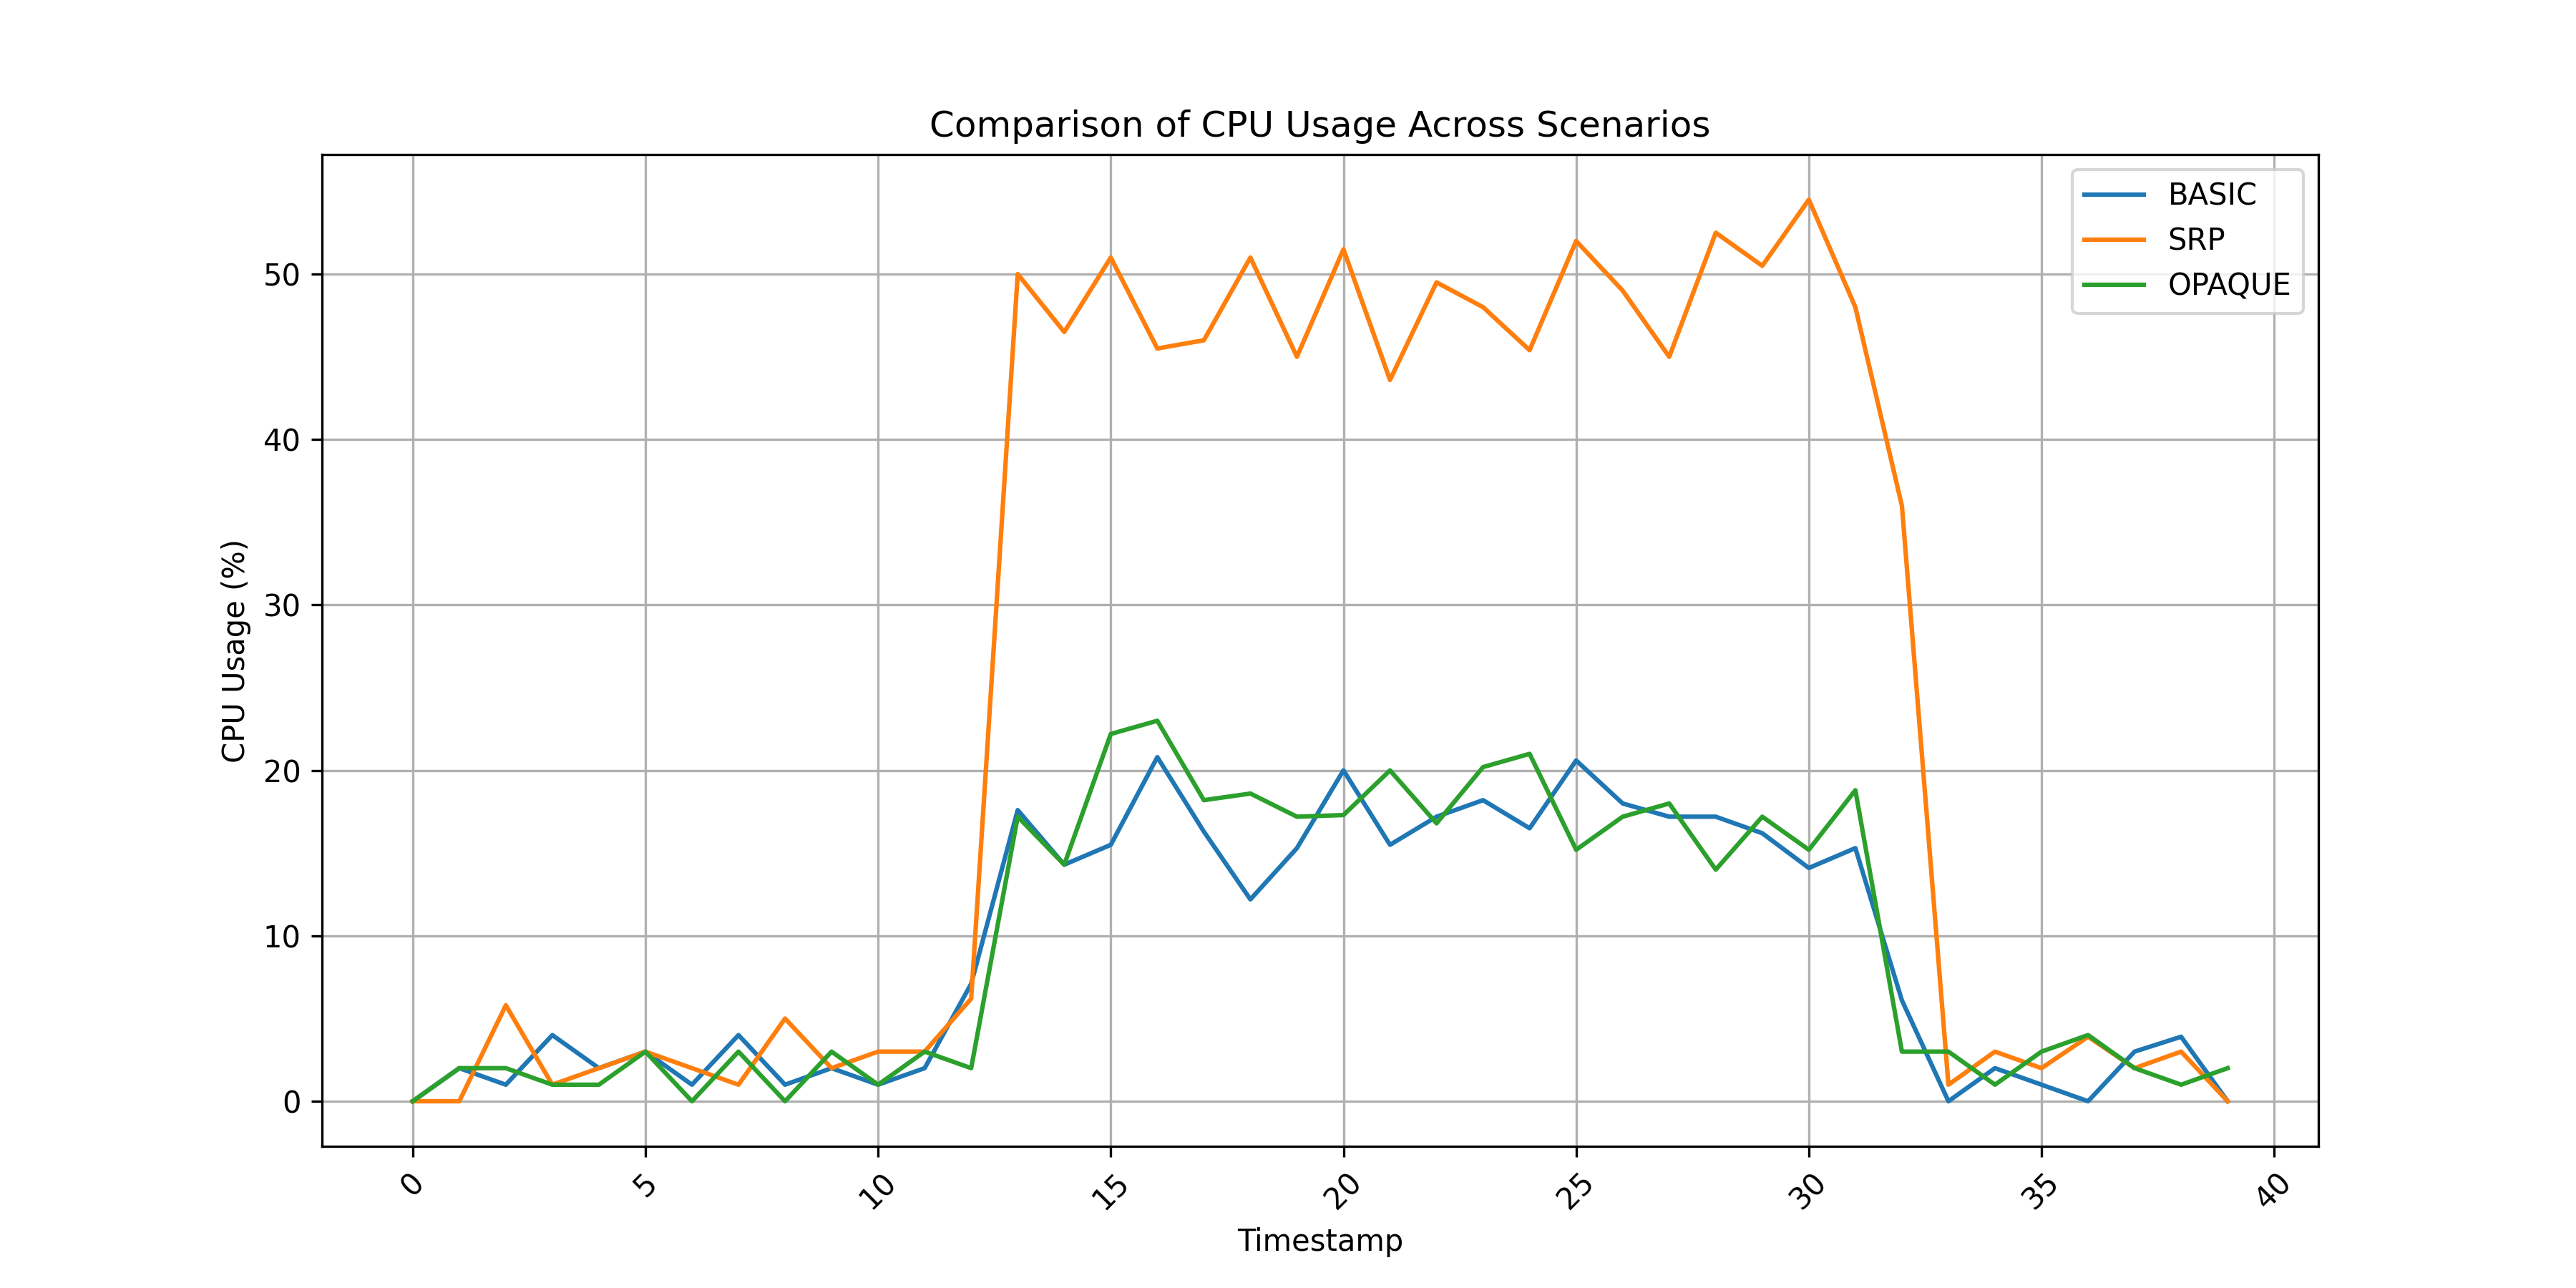
\includegraphics[width=0.4\textwidth]{./images/cpu_usage_comparison.png}
  \caption{Comparison of server-side CPU usage}
  \label{fig:cpu_usage}
\end{figure}

\subsection{Server-side CPU Usage}

One of the key performance metrics we examined was the server-side CPU utilization over time. The PAKE protocols, by nature, involve more complex cryptographic operations compared to a basic password-over-TLS authentication, which could potentially lead to higher CPU consumption.

The Password Over TLS protocol exhibited a relatively stable and low CPU usage throughout the experiment, as the server-side logic primarily involved hashing the password and comparing it to the stored value in the database.

In contrast, the SRP protocol demonstrated a much higher and more variable CPU usage over time. The server-side computations required for the SRP protocol, such as generating ephemeral keys and deriving the session proof, placed a significantly higher demand on the CPU resources. This could be a potential bottleneck for servers handling a large number of concurrent authentication requests.

The OPAQUE protocol also showed elevated CPU usage compared to Password Over TLS, but it was generally lower and more stable than the SRP protocol. The server-side operations in OPAQUE, such as the oblivious pseudorandom function (OPRF) and the encryption/decryption of the client's private key, appeared to be more efficiently implemented, leading to a more manageable CPU utilization.

\begin{figure}[ht]
  \centering
  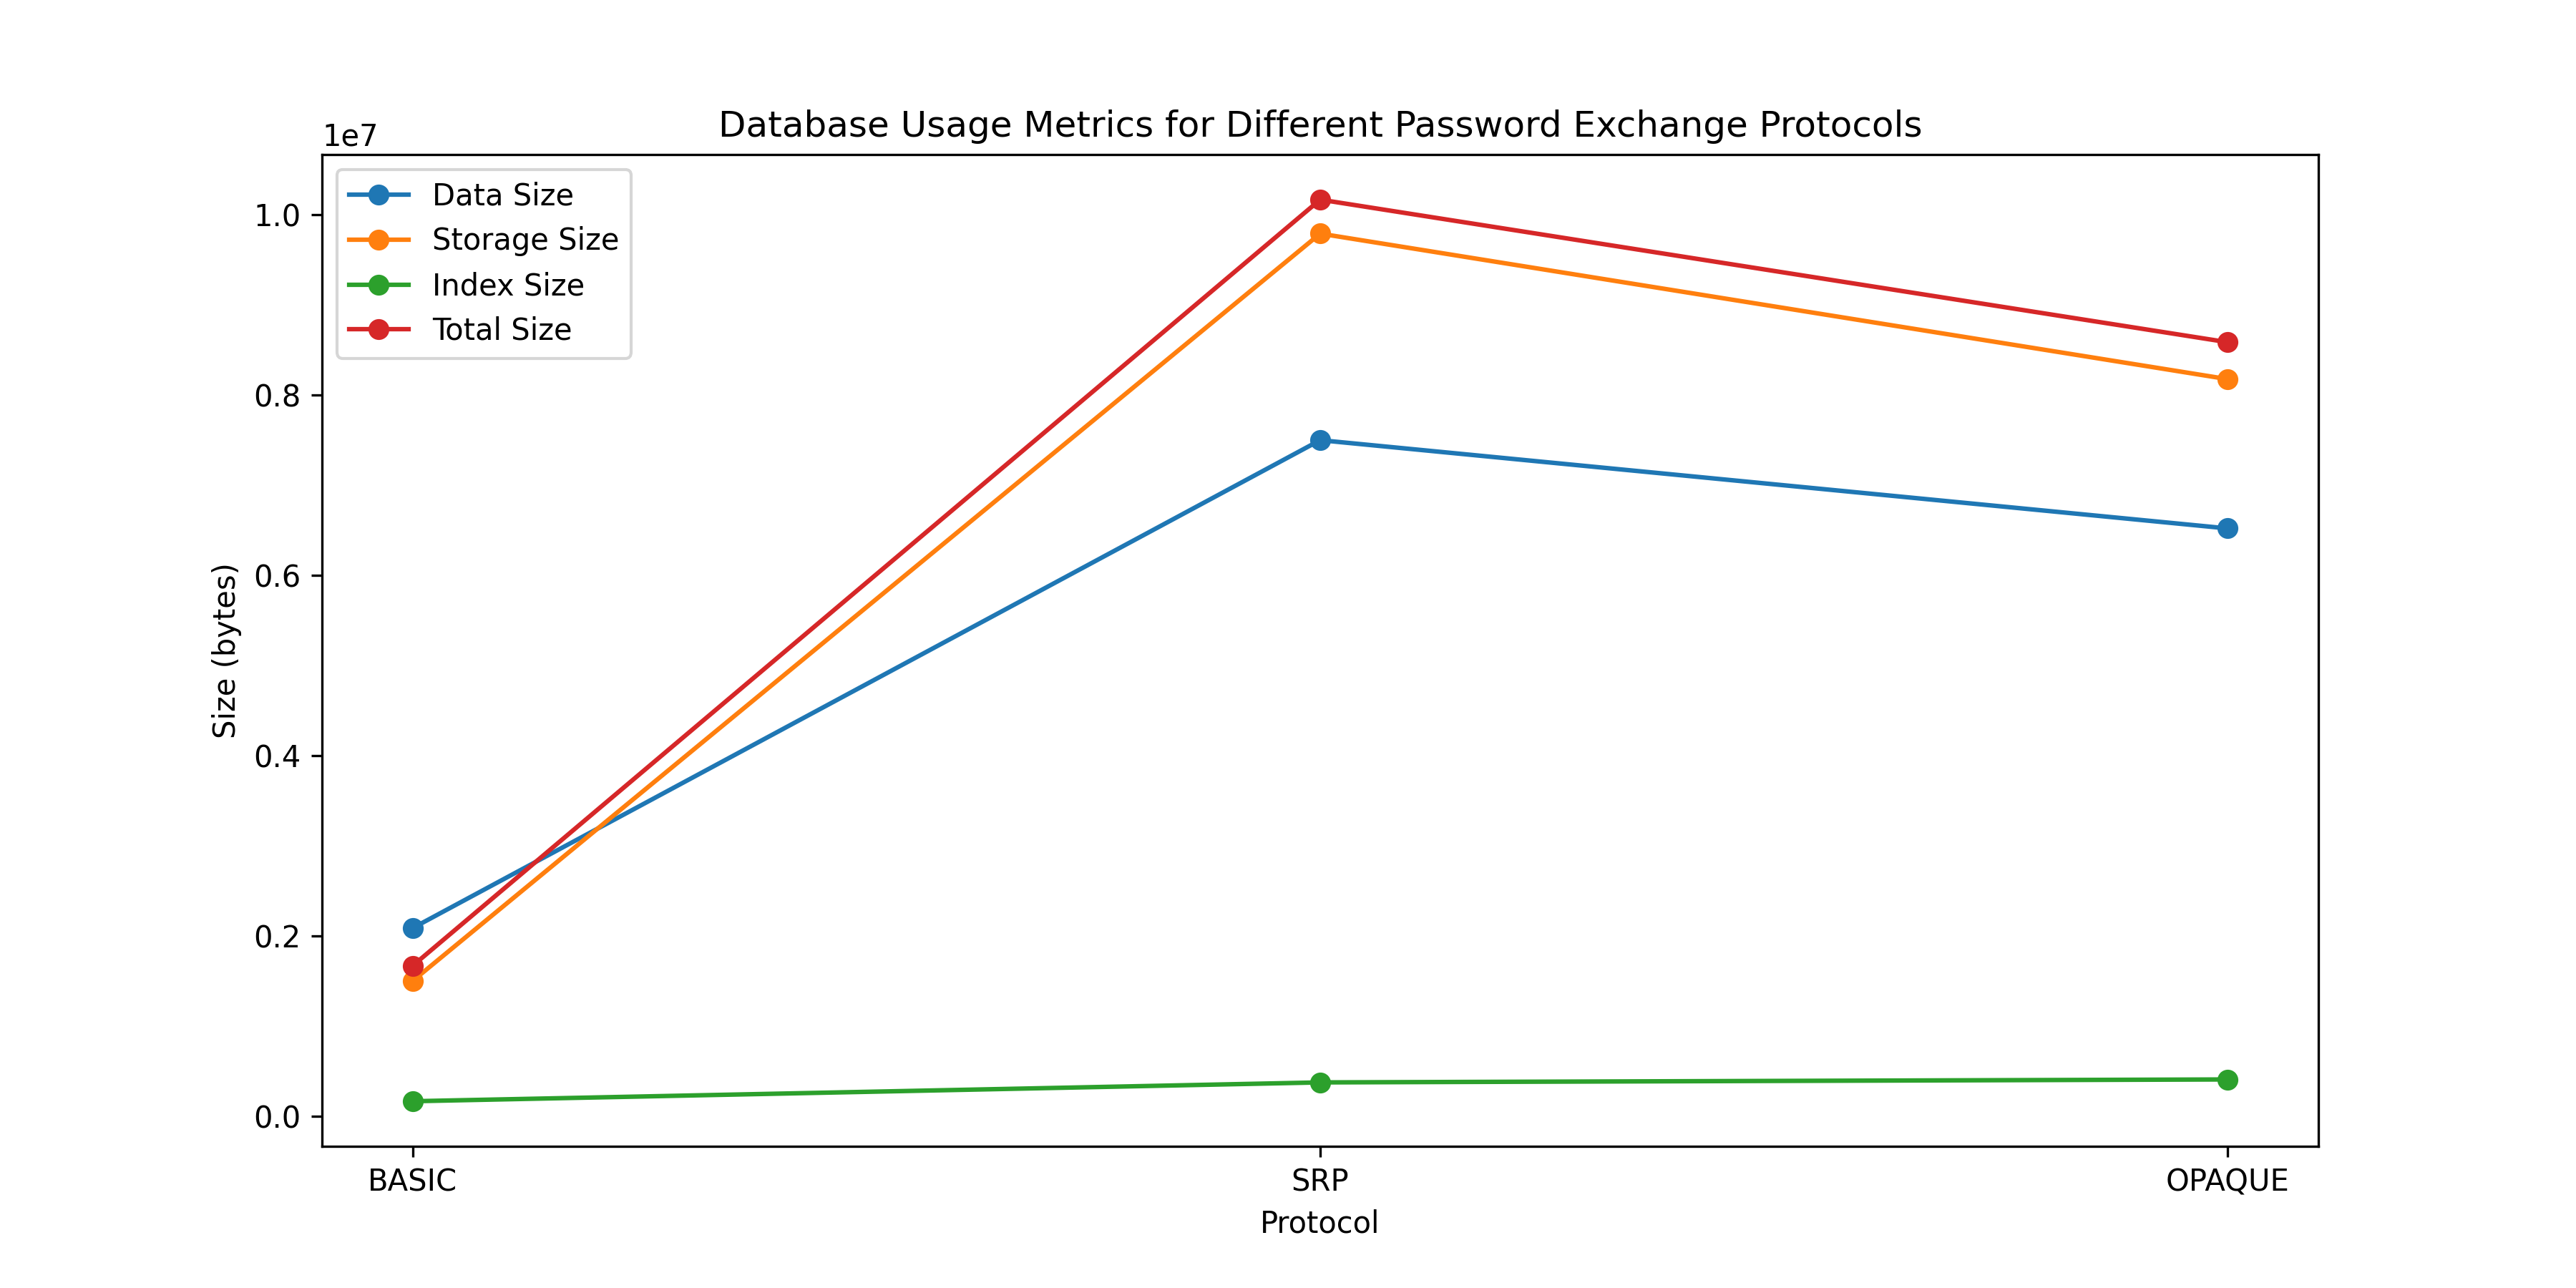
\includegraphics[width=0.4\textwidth]{./images/database_usage_metrics_line.png}
  \caption{Comparison of server-side storage usage}
  \label{fig:storage_usage}
\end{figure}

\subsection{Server-side Storage Usage}

Another aspect we investigated was the impact of the PAKE protocols on the server-side storage requirements. The storage usage is an important consideration, as PAKE protocols often require storing additional data, such as salts, session information, or encrypted client keys, to facilitate the authentication process.

Our experiments revealed that the PAKE protocols, in general, required more storage space compared to the basic password-over-TLS authentication. The SRP protocol and the OPAQUE protocol had roughly the same storage usage, with the SRP protocol being slightly higher.

For the SRP protocol, the server needed to store the user's username, the generated secret value (V), and the salt (s) for each registered user. This additional data overhead amounted to an increase in storage requirements compared to the baseline password-over-TLS protocol.

The OPAQUE protocol, on the other hand, required storing a more complex data structure, including the encrypted envelope (E) containing the client's private key, the client's public key (CKp), and the salt (s) specific to each user's username. The storage usage for the OPAQUE protocol was slightly lower than the SRP protocol, but still significantly higher than the baseline.

The Password Over TLS protocol, being the simplest in terms of server-side implementation, had the smallest storage footprint, as it only required storing the user's hashed password along with the salt. The storage usage for the Password Over TLS protocol was roughly half of the SRP and OPAQUE protocols.

\begin{figure}[ht]
  \centering
  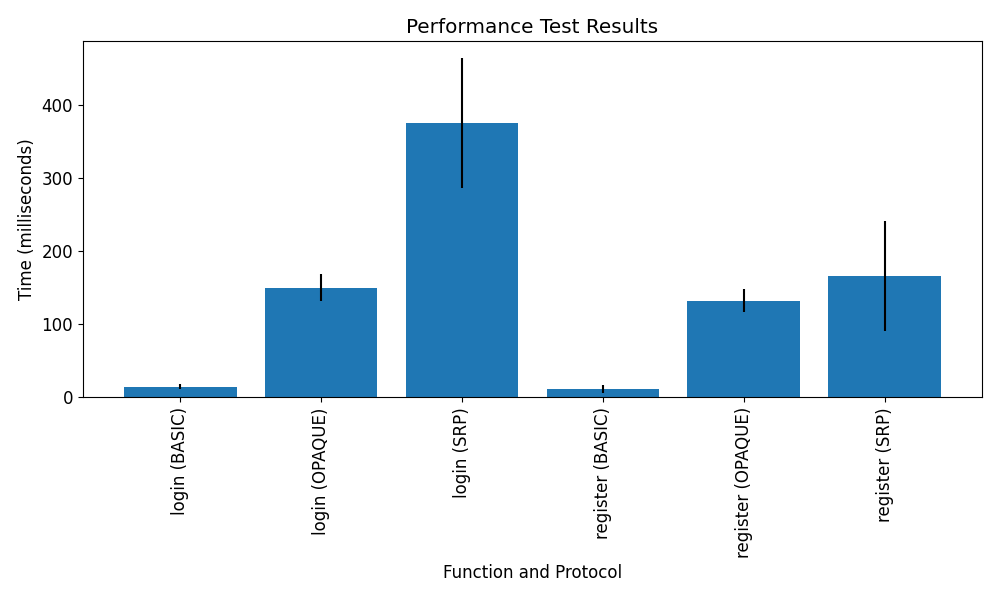
\includegraphics[width=0.4\textwidth]{./images/performance_test.png}
  \caption{Comparison of client-side per-request response times}
  \label{fig:performance_test}
\end{figure}

\subsection{Client-side experience}

In addition to the server-side performance metrics, we also examined the client-side experience during the authentication process. This was an important aspect to consider, as the user-perceived responsiveness and efficiency of the authentication flow can significantly impact the overall user experience.

The Password Over TLS (baseline) exhibited the fastest and most consistent response times throughout the simulation. The client-side request processing was relatively straightforward, involving the transmission of the username and password, followed by the server's verification and response. This simplicity translated to a smooth and responsive user experience, with minimal latency.

In contrast, the SRP protocol demonstrated significantly longer and more variable response times compared to Password Over TLS. The client-side implementation of SRP required a more complex series of message exchanges, including the generation of ephemeral keys, the computation of the session proof, and the verification of the server's response. This additional computational overhead and the back-and-forth communication between the client and server resulted in a less responsive user experience, with some requests taking considerably longer to complete.

The OPAQUE protocol also exhibited longer response times compared to Password Over TLS, but the overall performance was better than SRP. The client-side operations in OPAQUE, such as the oblivious pseudorandom function (OPRF) and the encryption/decryption of the client's private key, were more optimized than the SRP protocol, leading to a more consistent and responsive user experience. However, the response times for OPAQUE were still noticeably longer than the baseline Password Over TLS protocol.
\section{Questionnaire result}




The questionnaire remained open for a week, during which time it garnered responses from a total of 136 anonymous participants.
Since we shared the link out to friends and family, we are expecting the age distribution of the participants to be mainly around 18 to 25, with some participants reaching age 50 and above.
From our friend groups and family members, we assume all the participants to the questionnaire has basic knowledge to technology, such as navigate through websites or using social media.

\begin{figure}[ht]
  \centering
  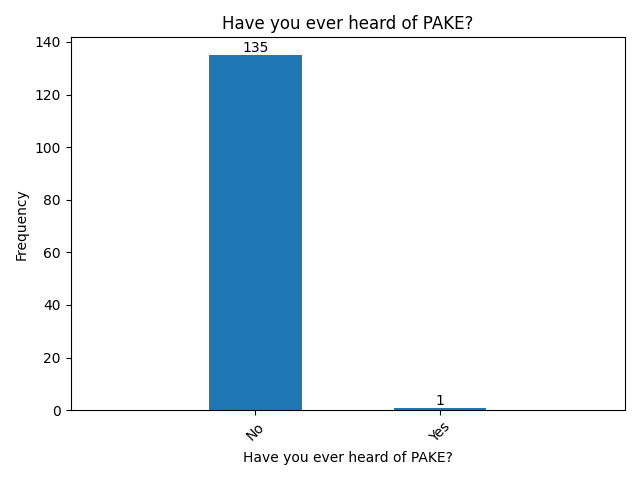
\includegraphics[width=0.4\textwidth]{./images/know_pake.png}
  \caption{Numbers of participants heard about PAKE}
  \label{fig:know_pake}
\end{figure}

\subsection{Knowledge about PAKE}
We asked the participants whether they have heard about PAKE protocols or not.
Initially, we did not expect any participants to know anything about PAKE, speaking from our experience that none of us knew PAKE until we start working on the project.
But surprisingly, one participant out of 136 actually knew about PAKE protocols with prior knowledge, as shown in ~\figref{fig:know_pake}.
They highlighted that "PAKE protocols use zero-knowledge proofs to authenticate without transmitting passwords. Good for security," which is the goal PAKE is aiming to achieve.





\begin{figure}[ht]
  \centering
  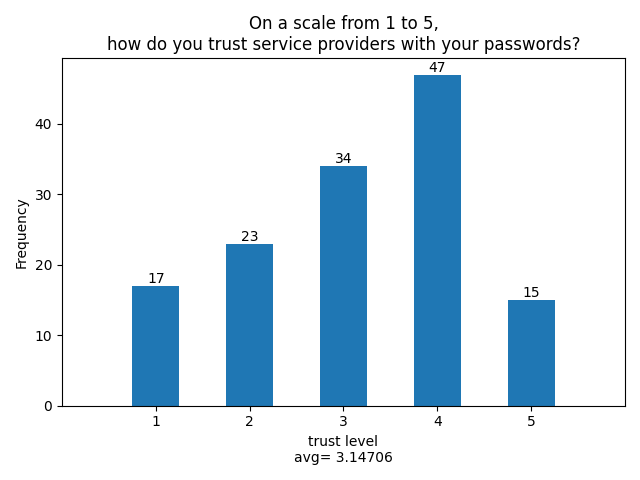
\includegraphics[width=0.4\textwidth]{./images/service_provider_trust.png}
  \caption{Trust towards service providers with participants' passwords.
    The intensity is measured on a scale of 1 to 5, where 1 represents not secure, and 5 represents very secure.}
  \label{fig:trust}
\end{figure}


\subsection{Trust to Password over TLS and service providers}
\label{sec:trust}
We are also curious how users trust service providers with their password.
We informed the participants that Password over TLS implementation requires storing encrypted password in the service providers' databases, and wanted to collect some feedback for this implementation.
Most answers surrounded the idea of data breach and leaks, which is one way an adversary gain control of a user's account.
One participant mentioned that "widely-used authentication methods, once subject to a data breach, are completely vulnerable: all users' data can be extracted, as user passwords are entirely stored on the server side databases."
While this is not entirely correct, storing password in server's database can add additional risks to lose all other personal data stored with the service provider.

Another participant mentioned password reusing, saying that most people would not bother to remember multiple passwords to different services, which can put all the services that use same password in danger if one of them is breached.
He also said in order to prevent the incident from happening, users often use password managers or notebook applications to keep track their passwords, but the additional use of programs brings another vulnerability to the potential leak of passwords.

Furthermore, we asked the participants whether they trust service providers with their passwords.
The result in ~\figref{fig:trust} shows that part of the uses are confident about their password being handled safely by the service providers, but at the same time, another part of the participants felt uncertain about the situation.
We can see a slightly right skewed trend from the figure, but we believe it is not significant enough to show whether a user trust the server would safe their passwords securely or not.
% From the average of the result, we did not see any significant tendency whether a user trust or is skeptical of the Password over TLS implementation.



\begin{figure}[ht]
  \centering
  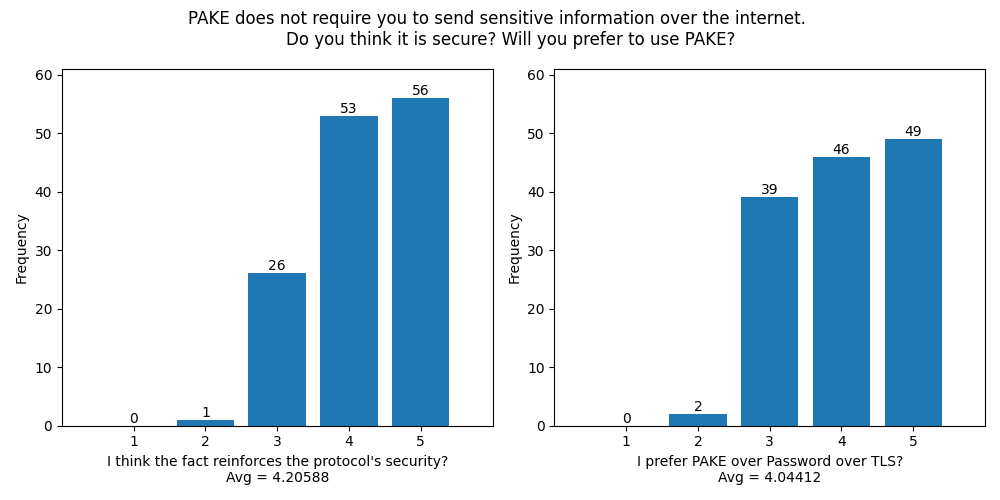
\includegraphics[width=0.4\textwidth]{./images/secure_preference.png}
  \caption{Participants' opinion on PAKE protocols. 
  The intensity is measured on a scale from 1 to 5, where 1 represents most unlikely, and 5 represents most likely}
  \label{fig:preference}
\end{figure}

\subsection{Preference between PAKE and Password over TLS}
\label{sec:preference}

In the questionnaire we stressed the point that PAKE protocols do not require passwords to be sent through the internet.
We would like to see how participants would response with this information, whether they think it is more secure or less.
From ~\figref{fig:preference}, it is apparent that the majority of participants view authentication methods that avoid transmitting passwords over the internet as more secure, and have a higher preference to embrace protocols that does not require transmitting.
% We can see such tendency are positively related to each other, 

In ~\secref{sec:trust}, participants pointed out some potential flaws Password over TLS have, but only a slight right skew on ~\figref{fig:trust} is observed.
% does not seem to have a common agreement on the trust towards service providers.
However, in ~\secref{sec:preference}, they showed high interest in using protocols that does not send sensitive information. 
We assume that the slight right skew comes from the trust towards big companies that most users think are reliable, but when an alternative that does not require sensitive data to be transmitted, users would opt for the second option to guard their security.

\begin{figure}[ht]
  \centering
  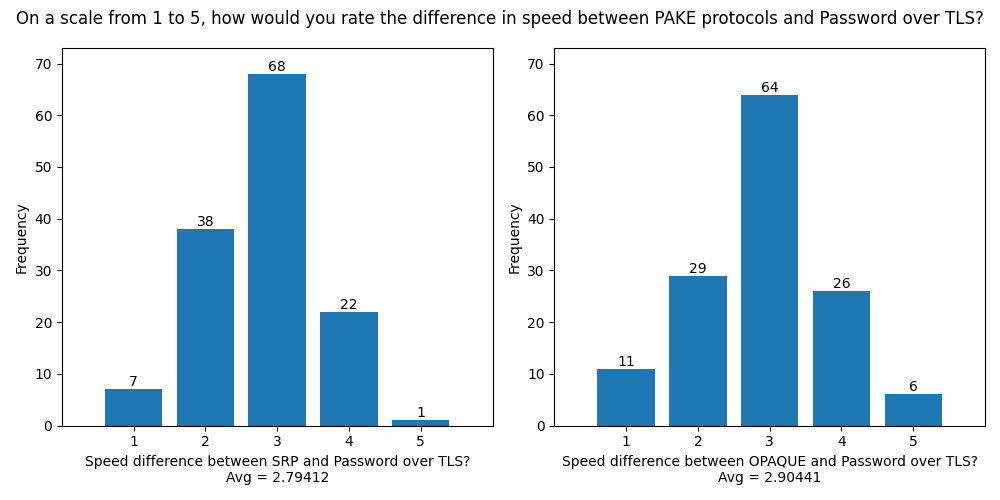
\includegraphics[width=0.4\textwidth]{./images/ux_compare.png}
  \caption{Response time difference between PAKE protocols and Password over TLS.
  The intensity is measured on a scale from 1 to 5, where 1 represents much slower, and 5 represents much faster.}
  \label{fig:compare}
\end{figure}

\subsection{User experience analysis}
We provided participants with access to the three implementations, enabling them to directly assess the variations in time consumption. 
Participants were then instructed to log in using all three services, assess their responsiveness, and make comparisons between the two PAKE protocols and the controlled Password over TLS implementation.
From ~\figref{fig:compare}, participants report similar time consumption when comparing both PAKE protocols to Password over TLS.

This raises our question about why PAKE is rarely implemented. 
Despite the minimal differences in user experience compared to Password over TLS, we anticipated increased adoption of PAKE across various platforms.
However, the reality contradicts our expectations.
We assume that developers chose not to implement PAKE protocols becuase the heavy workload that falls on the server side, showed in ~\secref{sec:exp_results}.
Also, PAKE implementations are much more complicated then Password over TLS, which requires much more effort to trace the logic when building the protocol and maintaining the system. 
\section{Conclusion}
\label{sec:conclusion}
A need of new authentication method rises since the vulnerability of Password over TLS rely heavily on the safety measurements made by server providers.
PAKE protocols leverage cryptographic techniques to ensure both client and server would not know any information other than success or failure in one login attempt.
Our goal is to evaluate the usability of two PAKE protocols, SRP and OPAQUE, of their possibility of deployment and user friendliness. 
To facilitate this, we developed three identical web services utilizing SRP, OPAQUE, and Password over TLS.
Each service includes a register and a login page to enable system-wide analysis, complemented by a user experience study conducted through a structured survey.

Our study revealed that the PAKE protocols, namely SRP and OPAQUE, incurred higher computational overhead on the server compared to the baseline password-over-TLS authentication. The SRP protocol exhibited significantly higher and more variable CPU usage over time, which could potentially be a bottleneck for servers handling a large number of concurrent authentication requests. The OPAQUE protocol, on the other hand, showed elevated but more stable CPU usage compared to SRP, suggesting better efficiency in its server-side implementation.

We think that the increased server-side resource utilization of the PAKE protocols is an important practical consideration for their deployment in real-world applications. While PAKE protocols provide stronger security guarantees by protecting the user's password from exposure, system administrators and decision-makers must carefully evaluate the tradeoffs between the security benefits and the potential performance impact on the server infrastructure. Optimizing the PAKE protocol implementations or adopting more efficient cryptographic primitives could help mitigate the performance challenges and make the deployment of PAKE-based authentication more feasible in high-load scenarios.

Additionally, the client-side experience revealed that the PAKE protocols, especially SRP, exhibited longer and more variable response times compared to the baseline password-over-TLS authentication. This could negatively impact the user experience, as users may perceive the authentication process as less responsive and efficient. Continued efforts to streamline the client-side operations and reduce the communication overhead between the client and server could help improve the user-perceived performance of PAKE-based authentication.

Moreover, the survey revealed that most of our participants has never heard of PAKE protocols, suggesting the opportunity for broader awareness regarding PAKEs.
Participants also showed much interest in PAKE protocols, due to the fact that PAKEs eliminated the need to transmit passwords over the internet and save them in service providers' databases.
This suggests that users are unlikely to be the primary reason for the limited adoption of PAKE protocols among various authentication methods.
Lastly, participants reported similar waiting time for the two PAKE protocols compared to Password over TLS.
This further supports our guess that the calculation work load required on server side is the reason why PAKE has not been widely implemented. 
We did not gather information regarding the device models participants utilized during their interaction with our implementation.
This oversight may serve as a factor influencing the potential variability in wait times observed for PAKE protocols.

We believe PAKE protocols hold promise for adoption in production environments. 
We anticipate that our contribution will help advance the integration of PAKEs into production systems.


%%% Local Variables:
%%% mode: latex
%%% TeX-master: "main"
%%% End:





\bibliographystyle{ACM-Reference-Format}
\bibliography{bib}

% --- Appendix ---%
\appendix
\section{Overflow form other sections}
\label{sec:set-diff-dodis}
Sometime you ware super excited about some details that does not quite fit with
the rest of the paper goes here. For example, some details about how you
instrumented the Android Linux kernel should go to appendix, and for really
curious reader to read. Remember it's appendix, so the reader is not required to
read, and you should not put critical information in appendix that is crucial
for understanding the rest of the paper.


\end{document}
